\documentclass{book}

\usepackage{graphicx}
\usepackage{xkeyval}
\usepackage{multirow}
%\usepackage{bm} %% bold face math symbols
\usepackage{listings}
\lstset{mathescape}
\usepackage{../macros/mytikz}
%\usepackage{multicol}
\usepackage{stmaryrd}%\newcommand{\contra}{\lightning}
%\usepackage{rotating} \newcommand{\sw}[1]{\begin{sideways}#1\end{sideways}}
\usepackage[show]{ed}
%\usepackage{../macros/algorithm}
%\usepackage{ded}

\usepackage{../mylecturenotes}
\usepackage{../macros}
\usepackage{local}
\usepackage{cleveref}

\title{Lectures Notes on Knowledge Representation and Processing}
\author{Florian Rabe and Michael Kohlhase}
\date{2022}

\begin{document}
\maketitle

\bigskip

These notes were originally prepared for our CS course at University Erlangen-Nuremberg (FAU) in Summer 2020.
They are directed at 3rd semester CS undergraduates and master students but should be intelligible even for earlier students and could be interesting also for PhD students and for students from adjacent majors.
The course is recommended both as a first course in the specialization area Artificial Intelligence as well as a one-off overview on on knowledge representation.

The course was developed in Summer 2020 from scratch and materials were built along the way.
It integrated current directions and recent results in research on knowledge representation pulling together materials in an entirely new and original way.

\tableofcontents

\newpage

%%%%%%%%%%%%%%%%%%%%%%%%%%%%%%%%%%%%%%%%%%%%%
\setcounter{chapter}{-1}
\chapter{Meta-Information}
 \section{Remarks}
  \input{../generalremarks}
\section{Overview}
  \paragraph{Structure}

The subsequent \emph{parts} of this course follow the Tetrapod model with one part per aspect.
Each of these will describe the concepts, languages, and tools of the respective aspect as well as their relation to other aspects.

The aspects of the Tetrapod are typically handled in individual courses, which describe highly specialized languages and tools in depth.
On the contrary, the overall goal of this course will be seeing all of them as different approaches to semantics and knowledge representation.
The course will focus on universal principles and their commonalities and differences as well as their advantages and disadvantages.

The subsequent \emph{chapters} of this first part will be dedicated to aspect-independent material.
These will not necessarily be taught in the order in which they appear in these notes.
Instead, some of them will be discussed in connection to how they are relevant in individual aspects.

\paragraph{Exercises and Running Example}

Typical practical projects, e.g., the ones that a strong CS graduate might be put in charge of, involve heterogeneous data and knowledge that must be managed using a variety of optimized aspect-specific languages and tools.
Interoperability between these is often a major source of inefficiency and bugs.

The exercises accompanying the course will mimic this situation: they will be designed around a single large project that requires choosing and integrating methods, languages, and tools from all aspects.

Concretely, this project will be the development of a univis-like system for a university.
It will involve heterogeneous data such as course and program descriptions, legal texts, websites, grade tables, and transcript generation code.

Over the course of the semester students will implement a completely functional system applying the lessons of the course.
This is very unusual and often impossible for other courses: as any university course must teach many different things from a wide area, it is rarely possible to find a project that requires many and only lessons from a single course.
Here KRP is special because its material pervades all aspects of system development.



\chapter{Fundamental Concepts}\label{sec:wuv:concepts}
  \section{Abbreviations}

\begin{center}
\begin{tabular}{lll}
knowledge representation and processing & KRP & the general area of this course \\
knowledge representation language & KRL & a languages used in KRP \\
knowledge representation tool & KRT & a tool implementing a KPL and processing algorithms for it
\end{tabular}
\end{center}

\section{Motivation}

\subsection{Knowledge}

Human knowledge pervades all sciences including computer science, mathematics, natural sciences and engineering.
That is not surprising: \enquote{science} is derived from the Latin word \enquote{scire} meaning \enquote{to know}.
Similarly, philosophy, from which all sciences derive, is named after the Greek words \enquote{philo} meaning loving and \enquote{sophia} meaning wisdom, and the common ending \enquote{-logy} is derived from Greek \enquote{logos} meaning word (i.\,e., a representation of knowledge).

In regards to knowledge, computer science is special in two ways:
Firstly, many branches of computer science need to understand KRP as a prerequisite for teaching computers to do knowledge-based tasks.
In some sense, KRP is the foundation and ultimate goal of all artificial intelligence.%
\footnote{Indeed, a major problem with the currently very successful machine learning-based AI technology is that it remains unclear when and how it does KRP. That can be dangerous because it leads to AI systems recommending decisions without being able to explain why that decision should be trusted.}
Secondly, modern information technology enables all sciences to apply computer-based KRP in order to vastly expand on the domain-specific tasks that can be automated.
Currently all sciences are becoming more and more computerized, but most non-CS scientists (and many computer scientists for that matter) lack a systematic education and understanding of IT-KRP.
That often leads to bad solutions when domain experts cannot see which KRP solutions are applicable or how to apply them.

\subsection{Representation and Processing}

It is no coincidence that this course uses the phrase \enquote{Representation and Processing}.
In fact, this is an instance of a universal duality.
Consider the following table of analogous concept pairs, which could be extended with many more examples:

\begin{center}
\begin{tabular}{ll}
\toprule
Representation & Processing \\
\midrule
Static & Dynamic \\
Situation & Change \\
Be & Become \\
Data Structures & Algorithms \\
Set & Function \\
State & Transition \\
Space & Time \\
\bottomrule
\end{tabular}
\end{center}

Again and again, we distinguish a static concept that describes/represents what a situation/state is and a dynamic concept that describes how it changes.
If that change is a computer doing something with or acting on that representation, we speak of \enquote{processing}.

It is particular illuminating to contrast KRP to the standard CS course on Data Structures and Algorithms (DA).%
\footnote{The course is typically called \enquote{Algorithms and Data Structures}, but that is arguably awkward because algorithms can only exist if there are data structure to work with. Compare my notes on that course in this repository, where I emphasize data structures much more than is commonly done in that course.}
Generally speaking, DA teaches the methods, and KRP teaches how to apply them.
Data structures are a critical prerequisite for representing knowledge.
But data structures alone do not capture what the data means (i.\,e., the knowledge) or if a particular representation makes any sense.
Similarly, algorithms are the critical prerequisite for processing knowledge.
But while algorithms can be systematically analyzed for efficiency, it is much harder to analyze if an algorithm processes knowledge correctly.
The latter requires understanding what the input and output data means.

Capturing knowledge in computers is much harder than developing data structures and algorithms.
It is ultimately the same challenge as figuring out if a computer system is working correctly --- a problem that is well-known to be undecidable in general and very difficult in each individual case.

%%%%%%%%%%%%%%%%%%%%%%%%%%%%%%%%%%%%%%%%%%%%%%%%%%%%%%%%%%%%%%%
\section{Components of Knowledge}

\subsection{Syntax and Semantics, Data and Knowledge}

Four concepts are of particular relevance to understanding knowledge.
They form a $2\times 2$-quadruple of concepts:

\begin{center}
\begin{tabular}{l|l}
Syntax & Data \\
\hline
Semantics & Knowledge
\end{tabular}
\end{center}

All four concepts are primitive, i.\,e., they cannot be defined in simpler terms.
All sciences have few carefully-chosen primitives on which everything builds.
This is done most systematically in mathematics (where primitives include set or function).
While mathematical primitives as well as some primitives in physics or CS are specified formally, the above four concepts can only be described informally, ultimately appealing to pre-existing human understanding.
Moreover, this description is not standardized --- different courses may use very different descriptions even if they ultimately try to capture the same elusive ideas.

\textbf{Data} (in the narrow sense of computer science) is any object that can be stored in a computer, typically combined with the ability to input/output, transfer, and change the object.
This includes bits, strings, numbers, files, etc.

Data by itself is useless because we would have no idea what to do with it.
For example, the object $O=((49.5739143, 11.0264941), "2020-04-21\text{T}16:15:00\text{CEST}")$ is useless data without additional information about its syntax and semantics.
Similarly, a file is useless data unless we know which file format it uses.

\textbf{Syntax} is a system of rules that describes which data is \textbf{well-formed}.
For $O$ above the syntax could be \enquote{a pair of (a pair of two IEEE double precision floating point numbers) and a string encoding of an time stamp}. 
For a file, the syntax is often indicated by the file name extension, e.\,g., the syntax of an \texttt{html} file is given in Section 12 of the current HTML standard\footnote{\url{https://html.spec.whatwg.org/multipage/}}.

Syntax alone is useless unless we know what the semantics, i.\,e., what the data means and thus how to correctly interpret and process the data.
For example, the syntax of $O$ allows to check that $O$ is well-formed, i.\,e., indeed contains two numbers and a timestamp string.
That allows rejecting ill-formed data such as $((49.5739143, 11.0264941), "\text{foo}")$.
The HTML syntax allows us to check that a file conforms to the standard.

\textbf{Semantics} is a system of rules that determines the meaning of well-formed data.
For example, ISO 8601 specifies that timestamp string refer to a particular date and time in a particular time zone.
Further semantics for $O$ might be implicit in the algorithms that produce and consume it: such as \enquote{the first component of the pair contains two numbers between $0$ and $180$ resp. $0$ and $360$ indicating latitude resp. longitude of a location on earth}.
Semantics might be multi-staged, and further semantics about $O$ might be that $O$ indicates the location and time of the first lecture of this course.
Similarly, Section 14 of the HTML standard specifies the semantics of well-formed HTML files by describing how they are to be rendered in a web browser.

\textbf{Knowledge} is the combining of some data with its syntax and semantics.
That allows applying the semantics to obtain the meaning of the data (if syntactically well-formed and signaling an error otherwise).
In computer systems,
\begin{compactitem}
 \item data is represented using primitive data (ultimately the bits provided by the hardware) and encodings of more complex data (bytes, arrays, strings, etc.) in terms of simpler ones,
 \item syntax is theoretically specified using grammars and practically implemented in programming languages using data structures,
 \item semantics is represented using algorithms that process syntactically well-formed data,
 \item knowledge is elusive and often emerges from executing the semantics, e.\,g., rendering of an HTML file.
\end{compactitem}

\subsection{Semantics as Syntax Transformation}

In order to capture knowledge better in computer systems, we often use two syntax levels: one to represent the data itself and another to represent the knowledge.
These can be seen as input and output data.
In that case, semantics is a function that translates from the data syntax to the knowledge syntax, and knowledge is the pair of the data and the result of applying the semantics.
The following table gives some examples.

\begin{center}
\begin{tabular}{lll}
\toprule
Data syntax & Semantics function & Knowledge syntax \\
\midrule
SPARQL query & evaluation & result set \\
SQL query & evaluation & result table \\
program & compiler & binary code \\
program expression & interpreter & result value \\ 
logical formula & interpretation in a model & mathematical object \\
HTML document & rendering & graphical representation \\
\bottomrule
\end{tabular}
\end{center}

Thus, the role of syntax vs.\ semantics may depend on the context: just like one function's output can be another function's input, one interpretation's knowledge can be another one's syntax.
For example, we can first compile a program into binary and then execute it to returns its value.

Such hierarchies of evaluation levels are very common in computer systems.
In fact, most state-of-the-art compilers are subdivided into multiple phases each further interpreting the output of the previous one.
Thus, if knowledge is represented in computers, it is invariably data itself but relative to a different syntax.

\subsection{Heterogeneity of Semantics and Knowledge}

While it is easy to design languages to represent data in general, it is very difficult to designing KRLs that capture the human-level quality of knowledge.
Over the last few decades, the KRP area in computer science has diversified into different subareas that approach this research problem in fundamentally different ways.
In fact, KRP in the very general sense of this course is usually not even studied by itself --- instead the subareas are so different, specialized, and large that they all sustain their respective university courses and research conferences.

This is related to the fact that the data naturally comes in fundamentally different forms such as graphs, arrays, tables in the sense of relational databases, programs in a programming language, logical formulas, or natural language texts.
We speak of \textbf{heterogeneous} data.
These different forms of data are supported by highly specialized KPTs: graph databases, array databases, relational databases, package databases for programming languages, theorem databases for logics (e.\,g., the Isabelle Archive of Formal Proofs), databases of research papers (such as the arXiv), and so on.

All of these are very successful for their respective kind of data.
And all of them include specifications of semantics and KP algorithms that implement this semantics.
But it can vary massively how the semantics is specified and implemented.
This has caused major practical problems for tool interoperability: many projects require data in multiple formats and algorithms from multiple tools.
But the respective tools are often islands that assume that all data is represented in the tool's language and users do not use outside tools.
Therefore, the import/export capabilities of the tools are often limited.

Moreover, transporting data across systems is usually ignorant of the semantics: while each tool takes relatively good care to implement the semantics correctly, there is much less certainty that the semantics is preserved when exchanging data across tools.
For a trivial example, consider a tool that measures length in inches vs.\ a tool that uses centimeters, both using floating point numbers for the data: if they exchange the data, i.\,e., just the numbers, they may miscommunicate the semantics.%
\footnote{Problems like this have been involved in major disasters such as the Mars Climate Orbiter.} 

This problem is not easy to fix though.
The heterogeneity of data and semantics is so extreme that it is, in some cases, an open theoretical problem how knowledge can be shared at all across tools.
The basic idea --- exchange the data in a way that preserves semantics --- can be difficult to implement if both tools use entirely different paradigms to specify semantics.

%%%%%%%%%%%%%%%%%%%%%%%%%%%%%%%%%%%%%%%%%%%%%%%%%%%%%%%%%%%%%%%
\section{The Tetrapod Model of Knowledge}

The Tetrapod model of knowledge is an ongoing research project by the instructors of this course.
A first publication was made in \cite{CFKR:tetrapod:19}.
The structure of this course will draw heavily on the Tetrapod model to get an overview of the different approaches to KPR and their interoperability problems.

\subsection{Five Aspects of Knowledge}

The Tetrapod model distinguishes five basic \textbf{aspects} of knowledge and KPR as described below.
For each aspect, there is a variety dedicated KRLs supported by highly optimized KPTs as indicated in the following table:

\begin{center}
\begin{tabular}{lll}
\toprule
Aspect & KRLs (examples) & KPTs (examples) \\
\midrule
ontologization & ontology languages (OWL), description logics (ALC) & reasoners, SPARQL engines (Virtuoso) \\
concretization & relational databases (SQL, JSON) & databases (MySQL, MongoDb) \\
computation & programming languages (C) & interpreters, compilers (gcc) \\
deduction & logics (HOL) & theorem provers (Isabelle) \\
narration & document languages (HTML, LaTeX) & editors, viewers \\
\bottomrule
\end{tabular}
\end{center}

\textbf{Ontologization} focuses on developing and curating a coherent and comprehensive ontology of concepts.
This focuses on identifying the central concepts in a domain and their relations.
For example, a medical ontology would define concepts for every symptom, disease, and medication and then define relations for which symptoms and medications are related to which disease.

Ontologies typically abstract from the knowledge: they standardize identifiers for the concepts and spell out some properties and relations but do not try to capture all details of the knowledge.
Well-designed ontologies can capture exactly what different KPTs must share and can thus serve as interoperability layers between them.

While organization can use ontology languages such as OWL or RDF, the inherent complexity of formal objects in computer science and mathematics usually requires going beyond general purpose ontology languages (similar to how the programming languages underlying computer algebra systems usually go beyond general purpose programming languages).

\textbf{Concretization} uses languages based on numbers, strings, lists, and records to obtain concrete representations of datasets in order to store and query their properties efficiently.
Because concrete objects are so simple and widely used, it is possible and common to build concrete datasets on top of general purpose data representation languages and tools such as JSON or SQL.

\textbf{Computation} uses specification and programming languages to represent algorithmic knowledge.

\textbf{Deduction} uses logics and theorem provers  to obtain verifiable correctness.

\textbf{Narration} uses natural language to obtain texts that are easy to understand for humans.
Because narrative languages are not well-standardized (apart from general purpose languages such as free text or \LaTeX), it is common to develop narrative libraries on top of ad-hoc languages that impose some formal structure on top of informal text, such as a fixed tree structure whose leafs are free text or a particular set of {\LaTeX} macros that must be used.
Narrative libraries can be classified based on whether entries are derived from publications (e.\,g., one abstract per paper in zbMATH) or mathematical concepts (e.\,g., one page per concept in $n$Lab).
%While these languages have multiple implementations, individual libraries usually involve specific encodings that are implemented only by a single tool.

%For example, an organization language might state only a function's type and properties.
%A computational treatment provides an efficient implementation, a deductive one proves the properties, a concretized one tables the function's values, and a narrative one documents the nature and purpose of the function.


\subsection{Relations between the Aspects}

The aspects can be visualized as the corners of tetrahedron with ontologization in the center and edges and faces representing solutions that mix two or three aspects as seen in Figure~\ref{fig:tetrapod}.

\begin{figure}[hbt]
\begin{center}
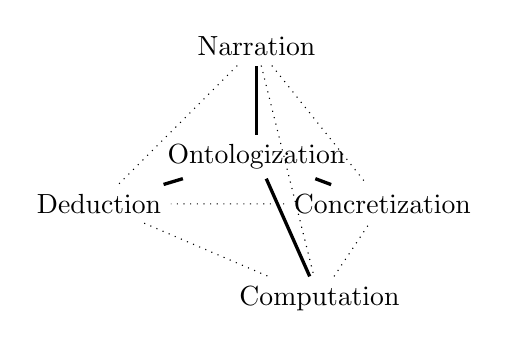
\begin{tikzpicture}[scale=4]
  \node (center) at (0,.15) {Ontologization};
  \node (left) at (.2,-.3) {Computation};
  \node (right) at (.4,0) {Concretization};
  \node (back) at (-.5,0) {Deduction};
  \node (up) at (0,.5) {Narration};

  \draw[very thick] (center) -- (left);
  \draw[very thick] (center) -- (right);
  \draw[very thick] (center) -- (back);
  \draw[very thick] (center) -- (up);
  \draw[dotted] (left) -- (right) -- (back) -- (left);
  \draw[dotted] (up) -- (left);
  \draw[dotted] (up) -- (right);
  \draw[dotted] (up) -- (back);
\end{tikzpicture}
\end{center}
\caption{Tetrapod model of knowledge}\label{fig:tetrapod}
\end{figure}

Most approaches try to incorporate all or multiple aspects.
But all languages and tools tend to be heavily biased towards and optimized for a single one of the four corner aspects.
This is not due to ignorance but because each aspect provides characteristic advantages that are extremely hard to capture at once.
In fact, every combination of aspects shares characteristic advantages and disadvantages as sketched in~\autoref{fig:tetrapod2}.
For example, deductive and narrative definitions of a function involved well-definedness arguments, and a function defined by a concrete table is trivially well-defined, but a computational definition of a function may throw exceptions when running; but only the latter can store and compute functions efficiently.
Consequently, dedicated and mostly disjoint communities have evolved that have produced large aspect-specific datasets.

\begin{table}[h]
\caption{Shared properties and advantages of aspects}\label{fig:tetrapod2}
\begin{subtable}{\textwidth}
\centering
\caption{Characteristics of aspects}
\begin{tabular}{lllp{2.8cm}l}
\toprule
	& \multicolumn{4}{c}{characteristic} \\
\cmidrule(lr){2-5}
Aspect &  objects & advantage & joint advantage of the other aspects & application \\
\midrule
deduction & formal proofs & correctness & ease of use & verification \\
computation & programs & efficiency & well-definedness & execution\\
concretization & concrete objects & tangibility & abstraction & storage/retrieval\\
narration & texts & flexibility & formal semantics & human understanding\\
\bottomrule
\end{tabular}
\end{subtable}

\medskip
\begin{subtable}{\textwidth}
\centering
\caption{Advantages of aspect pairs}
\begin{tabular}{ll}
\toprule
Aspect pair & characteristic advantage \\
\midrule
deduction/computation  & rich meta-theory \\
narration/concretization & simple languages \\
\addlinespace
deduction/narration  & theorems and proofs \\
computation/concretization & normalization \\
\addlinespace
deduction/concretization  & decidable well-definedness \\
computation/narration & Turing completeness \\
\bottomrule
\end{tabular}
\end{subtable}
\end{table}

%\subsection{Aspect-Specific Datasets in Mathematics}
%
%A survey of the state of the art in aspects is huge.
%Figure~\ref{fig:libraries} gives an overview of important datasets just the domain of mathematics.
%We have also pre-published a draft of an extensive survey in \cite{CarFarSharBerKohMueRab:somss20}.
%
%Crucially, these disjoint projects overlap massively.
%For example, the concept of \emph{group} is defined in most proof assistants and computer algebra systems, concrete groups are part of multiple large libraries (e.\,g., as the main object of interest in the small groups libraries, or as symmetry groups arising from other objects), and has entries in most narrative libraries (e.\,g., with entries in Stacks and nLab).
%Despite the overwhelming practical need, at the moment there is little to no technology to integrate libraries across this overlap.
%The same effect is found in other domains.
%
%\begin{figure}[ht]\centering\small\def\cite#1{}
%  \begin{tabular}{| p{.3\textwidth} | p{0.55\textwidth}|}\hline
%  Dataset & Description and approximate size \\\hline\hline
%  \multicolumn{2}{|l|}{\textbf{Inference}} \\\hline
%  Theorem prover libraries  & ??? \\\hline
%  \multicolumn{2}{|l|}{\textbf{Computation} \hfill\strut\hfill {\tiny CAS = computer algebra system}} \\\hline
%  Mathematica & commercial CAS, $5k$ built-in functions, $150$k official examples\\\hline
%  Maple & commercial CAS, $5$k built-in functions \\\hline
%  GAP \cite{gap} & CAS for group theory, $10$k statements \\\hline
%  Singular \cite{singular:on} & CAS for polynomials, over $90$ libraries \\\hline
%  SageMath \cite{SageMath:on} & $1$k modules, bundled with $4$GB of CAS tools and libraries\\\hline
%  Modelica \cite{Modelica:on} & modeling language, $5$k built-in classes, $100$ open source libraries, $50$ commercial libraries up to $0.5$M equations \\\hline\hline % $10$ official, $>100$ open-source, $50$ commercial,
%  \multicolumn{2}{|l|}{\textbf{Concretization}} \\\hline
% OEIS \cite{OEIS:on} & $330$k integer sequences, $1$ TB; $0.3$M sequence identities in \cite{kwarc:datahost:on} \\\hline
%%  OEIS identities \cite{kwarc:datahost:on} & $0.3$M sequence identities, $2.5$ TB \\\hline
% various databases of graphs\cite{ConderCensuses:on, HartleyPolytopes:on, LeemansPolytopes:on, PotocnikCensuses:on, RoyleVT:on, WilsonET:on} & highly symmetric graphs, maps, polytopes, $30$ datasets, $2$M objects, $1$TB \\\hline
%  various databases of lattices \cite{KohLat:on, LeeLat:on, MalLat:on} & $7$ datasets, $17$G objects, $1.5$ TB \\\hline
%  findstat \cite{findstat} & combinatorial statistics and maps, $1.5$k objects \\\hline
%  SageMath databases \cite{SageDB:on} & $12$ datasets \\\hline
%  $L$-functions and modular forms \cite{lmfdb:on} & $80$ datasets, $1$G objects, $1$ TB \\\hline
%  Small Groups Library \cite{BeEiOBSmallGroups} & $450$M groups, $80$ MB \\\hline\hline
%  \multicolumn{2}{|l|}{\textbf{Narration}\hfill\strut\hfill {\tiny based on publications (P) or concepts (C)}} \\\hline
%  arXiv.org (P) & $300$k math preprints, most with {\LaTeX} sources\\\hline
%  zbMATH \cite{zbMATH:on} (P) & $4$M publication abstracts with semantic data, $30$M reference data, $1$M disambig. authors, $2.7$M full text links \\\hline % $1$M OA 
%  EuDML  \cite{EuDML:on} (P) & $260$k open full-text publications, digitized journal back issues \\\hline
%%  MathOverFlow & $\approx 1,1$M questions/answers, $\geq11$K answer authors \\\hline
%  Stacks project (C) & $6$k pages, semantically annotated, curated, searchable textbook \\\hline
%  $n$Lab (C) & $13$k pages on category theory and applications\\\hline
%  SMGloM glossary (C) & $1$k modules, $2$k concepts, $4.5$k multi-lingual verbalizations in English \\\hline\hline %  (100\%), German (90\%), Chinese (10\%)
%  \multicolumn{2}{|l|}{\textbf{Organization}} \\\hline
%  swMATH \cite{swMATH:on} & $25$k software records with $300$k links to $180$k publications \\\hline
%  Wikidata  \cite{wikidata:on} & $34$GB linked data, $4$k formulas, interlinked with named theorems, persons, publications \\\hline
%  DLMF & $500$ special mathematical functions, $10$k formulas \\\hline
%  OpenMath CDs \cite{openmath} & curated reference points for $1.5$k concepts \\\hline
%  LATIN atlas \cite{CHKMR:latinabs:11,LATIN:online} & modular definitions of logics, $1$k modules \\\hline
%  Formal Abstracts  \cite{fabstracts} & formal definitions for all concepts used by multiple authors of mathematical papers (planned) \\\hline
%  \oaf interface library & as obtained in \oaf WP 2.6\\\hline
%\end{tabular}
%  \caption{Representative examples of large libraries by aspect}\label{fig:libraries}
%\end{figure}


\chapter{Representing Syntax and Semantics}\label{sec:wuv:syntax}
%\footnote{This chapter is grouped with the general parts to whom it belongs conceptually. But in the lecture it was treated later.}
  \section{Context-Free Syntax}

Abstractly, context-free syntax is specified using grammars.
Concretely, it is implemented using inductive types.

In the sequel, we will start with the standard definitions and then make a series of variation to each of these definitions until they become equivalent.
The intended equivalence is as follows:
\begin{center}
\begin{tabular}{l|l}
CFG & IDT \\
\hline
non-terminal & type \\
production & constructor \\
non-terminal on left of production & return type of constructor \\
non-terminals on right of production & arguments types of constructor \\
terminals on right of production & notation of constructor\\
words derived from non-terminal $N$ & expressions of type $N$
\end{tabular}
\end{center}

%%%%%%%%%%%%%%%%%%%%%%%%%%%%%%
\subsection{Context-Free Grammars}

We start with the usual definition:

\begin{definition}[Context-Free Grammar]
Given a set $\Sigma$ of characters (containing the terminal symbols), a \textbf{context-free grammar} consists of
\begin{compactitem}
\item a set $N$ of names called \textbf{non-terminal symbols}
\item a set of \textbf{productions} each consisting of
 \begin{compactitem}
  \item an element of $N$, called the \textbf{left-hand side}
  \item a word over $\Sigma\cup N$, called the \textbf{right-hand side}
 \end{compactitem}
\end{compactitem}
\end{definition}

\begin{example}
Let $\Sigma=\{0,1,+,\cdot,\doteq,\leq\}$.
We give a grammar for arithmetic expressions and formulas about them:
\begin{commgrammar}
\gprod{E}{0}{}\\
\galtprod{1}{}\\
\galtprod{E+E}{}\\
\galtprod{E\cdot E}{}\\
\gprod{F}{E\doteq E}{}\\
\galtprod{E\leq E}{}\\
\end{commgrammar}
Here we use the BNF style of writing grammars, where the productions are grouped by their left-hand side and written with $\bbc$ and $\bnfalt$.
We have $N=\{E,F\}$.
\end{example}

First, we give a name to each production of a CFG:

\begin{definition}[Context-Free Grammar with Named Productions]
Given a set $\Sigma$ of characters (containing the terminal symbols), a \textbf{context-free grammar} consists of
\begin{compactitem}
\item a set $N$ of names called \emph{non-terminal symbols}
\item a set of \emph{productions} each consisting of
 \begin{compactitem}
  \item a name
  \item an element of $N$, called the \textbf{left-hand side}
  \item a word over $\Sigma\cup N$, called the \textbf{right-hand side}
 \end{compactitem}
\end{compactitem}
\end{definition}

\begin{example}
The grammar from above with names written to the right of each production
\begin{commgrammar}
\gprod{E}{0}{zero}\\
\galtprod{1}{one}\\
\galtprod{E+E}{sum}\\
\galtprod{E\cdot E}{product}\\
\gprod{F}{E\doteq E}{equality}\\
\galtprod{E\leq E}{lessOrEqual}\\
\end{commgrammar}
This is not common BNF anymore.
\end{example}

Then we add base types to the productions:

\begin{definition}[Context-Free Grammar with Named Productions and Base Types]
Given a set $\Sigma$ of characters (containing the terminal symbols) and a set $T$ of names (containing the base types allowed in productions), a \textbf{context-free grammar} consists of
\begin{compactitem}
\item a set $N$ of names called \emph{non-terminal symbols}
\item a set of \emph{productions} each consisting of
 \begin{compactitem}
  \item a name
  \item an element of $N$, called the \textbf{left-hand side}
  \item a word over $\Sigma\cup T\cup N$, called the \textbf{right-hand side}
 \end{compactitem}
\end{compactitem}
\end{definition}

The intuition behind base types is that we commonly like to delegate some primitive parts of the grammar to be defined elsewhere.
A typical example are literals such as numbers $0, 1, 2,\ldots$: We could give regular expression syntax for digit-strings.
Instead, it is nicer to just assume we have a set of base types that we can use to insert an infinite set of literals into the grammar.

\begin{example}
Let $Nat$ be the type of natural numbers and let $T=\{Nat\}$.
Then we can improve the grammar from above as follows:
\begin{commgrammar}
\gprod{E}{Nat}{literal}\\
\galtprod{E+E}{sum}\\
\galtprod{E*E}{product}\\
\gprod{F}{E\doteq E}{equality}\\
\galtprod{E\leq E}{lessOrEqual}\\
\end{commgrammar}
\end{example}

%%%%%%%%%%%%%%%%%%%%%%%%%%%%%%
\subsection{Inductive Data Types}

We start with the usual definition:

\begin{definition}[Inductive Data Type]\label{def:idt}
Given a set of names $T$ (containing the types known in the current context), an \emph{inductive data type} consists of
\begin{compactitem}
 \item a name, called the \textbf{type},
 \item a set of \textbf{constructors} each consisting of
 \begin{compactitem}
  \item a name $n$
  \item a list of elements of $T\cup\{n\}$, called the \textbf{argument} types
 \end{compactitem} 
\end{compactitem}
\end{definition}

\newcommand{\cons}[2]{\mathtt{#1}\,\kw{of}\,\fold{*}{#2}}
\newcommand{\indtype}[2]{#1\,=\,\fold{\;\tb|\tb}{#2}}
\newcommand{\consnot}[3]{\mathtt{#1}\,\kw{of}\,\fold{*}{#2}\,\#\,#3}
\newcommand{\consn}[2]{\mathtt{#1}\,\#\,#2}

\begin{example}
Let $Nat$ be the type of natural numbers and $T=\{Nat\}$.
We give an inductive type for arithmetic expressions:
\[
\indtype{E}{\cons{literal}{Nat}, \cons{sum}{E,E}, \cons{product}{E,E}} \\
\]
Here we use ML-style notation for inductive data types, which separates constructors by $|$ and writes them as \texttt{name of argument-type-product}.
\end{example}

First we generalize to mutually inductive types:

\begin{definition}[Mutually Inductive Data Types]
Given a set $T$ of names (containing the types known in the current context), a family of \textbf{mutually inductive data type} consists of
\begin{compactitem}
 \item a set $N$ of names, called the \textbf{types},
 \item a set of \emph{constructors} each consisting of
 \begin{compactitem}
  \item a name
  \item an element of $N$, called the \textbf{return type}
  \item a list of elements of $N\cup T$, called the \textbf{argument} types
 \end{compactitem} 
\end{compactitem}
\end{definition}

\begin{example}
We extend the type definition from above by adding a second type for formulas.
Thus, $N=\{E,F\}$.
\[\mathll{
\indtype{E}{\cons{literal}{Nat}, \cons{sum}{E,E}, \cons{product}{E,E}} \\
\indtype{F}{\cons{equality}{E,E}, \cons{lessOrEqual}{E,E}}
}\]
\end{example}

%It may look $T$ and $\Sigma$ correspond to each other.
%But that is not true, we need to add them to each definition.

Then we add notations to the constructors:

\begin{definition}[Mutually Inductive Data Types with Notations]
Given a set $\Sigma$ of characters (containing the terminal symbols) and a set $T$ of names (containing the types known in the current context), a family of \textbf{mutually inductive data type with notations} consists of
\begin{compactitem}
 \item a set $N$ of names, called the \textbf{types},
 \item a set of \emph{constructors} each consisting of
 \begin{compactitem}
  \item a name
  \item an element of $N$, called the \textbf{return type}
  \item a list of elements of $T\cup N$, called the \textbf{argument} types
  \item a word over the alphabet $\Sigma\cup T\cup N$ containing the argument types in order and only elements from $\Sigma$ otherwise, called the \textbf{notation} of the constructor
 \end{compactitem} 
\end{compactitem}
\end{definition}

The intuition behind notations is that it can get cumbersome to write all constructor applications as $Name(arguments)$.
It is more convenient to attach a notation to them such as 

\begin{example}
We extend the type definitions from above by adding notations to each constructor.
We use the set $\Sigma=\{+,\cdot,\doteq,\leq\}$ as terminals in the notations.
\[\mathll{
\indtype{E}{\consnot{literal}{Nat}{Nat}, \consnot{sum}{E,E}{E+E}, \consnot{product}{E,E}{E\cdot E}} \\
\indtype{F}{\consnot{equality}{E,E}{E\doteq E}, \consnot{lessOrEqual}{E,E}{E\leq E}}
}\]
Here we write the constructors as \texttt{name of argument-type-product \# notation}.
It is easy to see that this has introduced redundancy: we can infer the argument types from the notation.
So we can just drop the argument types:
\[\mathll{
\indtype{E}{\consn{literal}{Nat}, \consn{sum}{E+E}, \consn{product}{E\cdot E}} \\
\indtype{F}{\consn{equality}{E\doteq E}, \consn{lessOrEqual}{E\leq E}}
}\]
\end{example}


\subsection{Merged Definition}

With the variation from above we have arrived at the following equivalence:

\begin{theorem}
Given a set $\Sigma$ of characters and a set $T$ of names, the following notions are equivalent:
\begin{compactitem}
\item a family of mutually inductive data types in the context of types $T$ with notations using characters from $\Sigma$,
\item a context-free grammar with named productions, terminal symbols from $\Sigma$, and base types $T$.
\end{compactitem}
\end{theorem}
\begin{proof}
The key idea is that
\begin{compactitem}
 \item the types and constructors of the former correspond to the non-terminals and productions of the latter
 \item for each constructor-production pair
  \begin{compactitem}
   \item the right-hand side of the latter corresponds to the notation of the former,
   \item the argument types of the former correspond to the non-terminals occurring on the right-hand side of the latter.
  \end{compactitem}
\end{compactitem}
\end{proof}

In implementations in programming languages, we often drop the notations.
Instead, those are handled, if needed, by special parsing and serialization functions.

However, in an implementation, it is often helpful to additionally give names to each argument of a production/constructor.
That yields the following definition:

\begin{definition}[Context-Free Syntax]
Given a set $\Sigma$ of characters and a set $T$ of names, a context-free syntax consists of
\begin{compactitem}
 \item a set $N$ of names, called the \textbf{non-terminals/types},
 \item a set of \textbf{productions/constructors} each consisting of
 \begin{compactitem}
  \item a name
  \item an element of $N$, called the \textbf{left-hand side/return type}
  \item a sequence of objects, called the \textbf{right-hand side/arguments} which are one of the following
   \begin{compactitem}
    \item an element of $\Sigma$
    \item a pair written $(n:t)$ of a name $n$, called the \textbf{argument name}, and an element $t\in T\cup N$ called the \textbf{argument type}.
   \end{compactitem}
 \end{compactitem}
\end{compactitem}
\end{definition}

\begin{example}
Using ad hoc language to write the constructors, our example from above as a context-free syntax could look as follows:
\[\mathll{
\indtype{E}{\consn{literal}{(value:Nat)}, \consn{sum}{(left:E)+(right:E)}, \consn{product}{(left:E)\cdot (right:E)}} \\
\indtype{F}{\consn{equality}{(left:E)\doteq (right:E)}, \consn{lessOrEqual}{(left:E)\leq (right:E)}}
}\]
\end{example}

\subsection{Contexts}

We assume a context-free language $l$.

\begin{definition}[Context]
A \textbf{context} is a list of
\begin{compactitem}
\item grammar terminology: productions $N\bbc x$
\item type terminology: declarations $x:N$
\end{compactitem}
where each $x$ is a unique name and each $N$ is non-terminal symbol.

The $x$ are called \textbf{variables}.
\end{definition}

\begin{remark}
Sometimes the grammar itself has specific productions for contexts and variables.
In that case, we speak of \emph{meta-variable contexts} and \textbf{meta-variables} to distinguish them from those of the language.
\end{remark}

\begin{definition}[Expressions in Context]
Given a context $\Gamma$, a word $E$ derived from non-terminal $N$ that may additionally use the productions of the context is called an \emph{expression of type} $N$ \emph{in context} $\Gamma$.

We write this as $\Gamma\vdash_l E:N$.
\end{definition}

\begin{definition}[Substitution]
Given two contexts $\vdash_l \Gamma$ and $\vdash_l\Delta$, a \textbf{substitution} $\gamma$ from $\Gamma=x_1:N_1,\ldots,x_n:N_n$ to $\Delta$ is a list $x_1:=e_1,\ldots,x_n:=e_n$ where every $e_i$ is an expression of type $N_i$ in context $\Delta$ (i.e., $\Delta\vdash_l e_i:N_i$).

We write this as $\Delta\vdash_l \gamma:\Gamma$ or as $\vdash_l \gamma:\Gamma\to \Delta$.
\end{definition}

\begin{definition}[Substitution Application]\label{def:subapp}
Given an expression $\Gamma\vdash_l E:N$ and a substitution $\vdash_l\gamma:\Gamma\to\Delta$ where $\Gamma=x_1:N_1,\ldots,x_n:N_n$ and $\gamma=x_1:=e_1,\ldots,x_n:=e_n$, we write $E[\gamma]$ for the result of replacing every $x_i$ in $E$ with $e_i$.
\end{definition}

\begin{theorem}
If $\Gamma\vdash_l E:N$ and $\vdash_l\gamma:\Gamma\to\Delta$, then $\Delta\vdash_l E[\gamma]:N$.
\end{theorem}

We often want to substitute only a single variable $x:N$ even though $E$ may be defined in a larger context $\Gamma$.
This is often written $E[x:=e]$.
That is just an abbreviation for $E[\gamma]$, where $\gamma$ contains $x:=e$ as well as $y:=y$ for every other variable $y$ of $\Gamma$.

\begin{notation}
There are many different notations for substitutions that are in common use.
Examples include $E(x)$, $E[x:=e]$, $E[x/e]$, or $[e/x]E$.
Usually authors of a paper or textbook briefly mention their preferred notation briefly at the beginning.
\end{notation}

\section{Implementation}

Context-free syntax can be implemented systematically in all programming languages.
But, depending on the style of the language, they make drastically different.
We give the two most important paradigms as examples.

\subsection{Functional Programming Languages}

In a function programming language, inductive data types are a primitive feature.
However, notations and named arguments are not available.
So helper functions must be used.

The basic recipe is as follows:
\begin{compactitem}
\item The types and constructors (without the notations and named arguments) are implemented as family of mutually inductive data types.
\item For each argument of each constructor, a partial projective function is defined.
\item A set of mutually recursive string rendering functions are defined, one for each constructor, that implement the notations.
\end{compactitem}

\begin{example}
We define our example syntax in ML.

First the inductive types (assuming a type $Nat$ already exists in the context):
\[\mathll{
\kw{data}\, \indtype{E}{\cons{literal}{Nat}, \cons{sum}{E,E}, \cons{product}{E,E}} \\
\kw{and}\,\indtype{F}{\cons{equality}{E,E}, \cons{lessOrEqual}{E,E}}
}\]

Now the projection functions:
\[\mathll{
 \kw{fun}\; \mathtt{literal\_value}(\mathtt{literal}(v)) = SOME\; v \\
 |\tb \mathtt{literal\_value}(\_)= NONE \\
 \kw{fun}\; \mathtt{sum\_left}(\mathtt{sum}(x,\_)) = SOME\; x \\
 |\tb \mathtt{sum\_left}(\_)= NONE\\
 \kw{fun}\; \mathtt{sum\_right}(\mathtt{sum}(\_,x)) = SOME\; x \\
 |\tb \mathtt{sum\_right}(\_)= NONE
}\]
and so on for each constructor argument.

Finally, the string rendering functions (assuming a function $natToString$ already exists in the context):
\[\mathll{
 \kw{fun}\; \mathtt{E\_toString}(\mathtt{literal}(v)) = natToString\;v \\
 |\tb \mathtt{E\_toString}(\mathtt{sum}(x,y))= \mathtt{E\_toString}(x) + "+" + \mathtt{E\_toString}(y) \\
 |\tb \mathtt{E\_toString}(\mathtt{product}(x,y))= \mathtt{E\_toString}(x) + "\cdot" + \mathtt{E\_toString}(y) \\
 \kw{and}\; \mathtt{F\_toString}(\mathtt{equality}(x,y)) = \mathtt{E\_toString}(x) + "\doteq" + \mathtt{E\_toString}(y)\\
 |\tb \mathtt{F\_toString}(\mathtt{lessOrEqual}(x,y)) = \mathtt{E\_toString}(x) + "\leq" + \mathtt{E\_toString}(y)
}\]
\end{example}

Because ML has inductive data types as primitives, pattern-matching on our syntax comes for free.
We will get back to that when defining the semantics.

\subsection{Object-Oriented Programming Languages}

In a object-oriented programming language, inductive data types are not available.
Therefore, they must be mimicked using classes.
On the positive side, this supports arguments names, and notations are a bit easier.

The basic recipe is as follows:
\begin{compactitem}
\item Each type is implemented as an abstract class.
\item Each constructor of type $t$ is implemented as a concrete class that extends the abstract class $t$.
\item The arguments names and type of each constructor $c$ are exactly the argument names and types of the class $c$.
The constructor arguments are stored as fields in the class.
\item The abstract classes require a \texttt{toString} method, which is implemented in every concrete class according to its notation.
\end{compactitem}


\begin{example}
We define our example syntax in a generic OO-language somewhat similar to Scala.\footnote{We could use Java or C++ here. But their concrete syntax makes this less clear than it could be. It is straightforward to refine the syntax into that of any specific OO-language.}

In particular, we assume that the sy

\begin{lstlisting}
abstract class E {
  def toString: String
}
class literal extends E {
  field value: Nat
  constructor (value: Nat) {
    this.value = value
  }
  def toString = value.toString
}
class sum extends E {
  field left: Nat
  field right: Nat
  constructor (left: E, right: E) {
    this.left = left
    this.right = right
  }
  def toString = left.toString + "+" + right.toString
}
class product extends E {
  field left: Nat
  field right: Nat
  constructor (left: E, right: E) {
    this.left = left
    this.right = right
  }
  def toString = left.toString + "$\cdot$" + right.toString
}

abstract class F {
  def toString: String
}
class equality extends E {
  field left: Nat
  field right: Nat
  constructor (left: E, right: E) {
    this.left = left
    this.right = right
  }
  def toString = left.toString + "$\doteq$" + right.toString
}
class product extends E {
  field left: Nat
  field right: Nat
  constructor (left: E, right: E) {
    this.left = left
    this.right = right
  }
  def toString = left.toString + "$\leq$" + right.toString
}
\end{lstlisting}
\end{example}

Because OO-languages do not have inductive data types as primitives, pattern-matching on our syntax requires awkward switch statements.
We will get back to that when defining the semantics.

\subsection{Combining Paradigms}

The Scala language combines ideas from functional and OO-programming.
That makes its representation of context-free syntax particularly elegant.

In Scala, the constructor arguments are listed right after the class name.
These are automatically fields of the class, and a default constructor always exists that defines those fields.
That gets rid of a lot of boilerplate.

If we want to make those fields public (and we do because those are the projection functions, we add the keyword \texttt{val} in front of them.
But even that is too much boilerplate. So Scala defines a convenience modifier: if we put \texttt{case} in front of the classes corresponding to constructors of our syntax, Scala puts in the \texttt{val} automatically.
It also generates a default implementation of \texttt{toString}, which we have to override if we want to implement notations, too.
Finally, Scala also generates pattern-matching functions so that we can pattern-match in the same way as in ML.

Then our example becomes (as usual, assuming a class \texttt{Nat} already exists):

\begin{lstlisting}
abstract class E {
  def toString: String
}
case class literal(value: Nat) extends E {
  override def toString = value.toString
}
case class sum(left: Nat, right: Nat) extends E {
  override def toString = left.toString + "+" + right.toString
}
case class product(left: Nat, right: Nat) extends E {
  override def toString = left.toString + "$\cdot$" + right.toString
}

abstract class F {
  def toString: String
}
case class equality(left: Nat, right: Nat) extends E {
  override def toString = left.toString + "$\doteq$" + right.toString
}
case class lessOrEqual(left: Nat, right: Nat) extends E {
  override def toString = left.toString + "$\leq$" + right.toString
}
\end{lstlisting}

\subsection{Issues Regarding Equivalence}

There are a few subtle issues.

\paragraph{Equality}
Forming the same value twice should yield the same result, e.g., $\mathtt{literal}(1)=\mathtt{literal}(1)$.
In ML-style inductive types, that is automatic.
In OO-style class-based implementations, we have $\kw{new}\,\mathtt{literal}(1)=\kw{new}\,\mathtt{literal}(1)$ only if we override the equality check.
Scala allows adding the keyword \kw{case} to a class representing a constructor/production.
Among other things, it allows dropping the \kw{new} and overrides the equality method automatically. 

\paragraph{Null Value}
Object-oriented language automatically provide the \cn{null} value for every class.
Therefore, if we implement a context-free syntax via classes, we always get one spurious value that should not exist.
Programmers have to use programming discipline to avoid using it.
Occasionally, static analysis tools can non-null annotations to check this discipline.

\paragraph{Sealing}
When we seal a context-free syntax, it is impossible to add new constructors to it.
That guarantees implementors of inductive functions that they know all possible cases and can therefore pattern-match on them.
An inductive function on an unsealed datatype can fail when new constructors are added later.

ML-style inductive data types are always sealed.
OO-style class-based implementations are never sealed.
In Scala, the keyword \kw{sealed} can be added to an abstract class --- it forbids any constructors other than the ones present in the same source file.


%The equivalence is as follows:
%\begin{center}
%\begin{tabular}{l|l}
%syntax & case-based function & recursive function \\
%\hline
%non-terminal $N$ & function $N$ & function with input $x:N$\\ 
%production & constructor \\
%non-terminal on left of production & return type of constructor \\
%non-terminals on right of production & arguments types of constructor \\
%terminals on right of production & notation of constructor
%\end{tabular}
%\end{center}


\section{Context-Sensitive Syntax}

It is common to define a language as the set of words that can be produced from the syntax, i.e., from a distinguished non-terminal (the start symbol) of the context-free grammar.
It is common to define a context-sensitive language as a special case: the set of words that can be produced from a context-sensitive grammar.

This is, however, not helpful in practice.
While the above remains the official definition of what the context-sensitive languages are, all practical definitions are entirely different.
In fact, context-sensitive grammars are virtually never used to define a specific language.
Instead, more restrictive definitions are used that capture more properties of practical languages.
In the sequel, we give one possible definition.\footnote{This definition works well in the context of this lecture but is non-standard. There is no standard definition at all. Instead, various similar definitions exist.}

\begin{definition}
A \textbf{language system} consists of
\begin{compactitem}
 \item a context-free syntax,
 \item a distinguished non-terminal symbol $\ThySym$, whose words are called \textbf{vocabularies},
 \item a set of distinguished non-terminal symbols $\ExpSym$, whose words are called $\ExpSym$-\textbf{expressions},
 \item a unary predicate $\wft{\Theta}$ on vocabularies $\Theta$,
 \item for every vocabulary $\Theta$ and every $\ExpSym$, a unary predicate $\wff{\Theta}{\ExpSym}{E}$ on $\ExpSym$-expressions $E$.
\end{compactitem}

In case of $\wft{\Theta}$, we call $\Theta$ \textbf{well-formed}.
In case of $\wff{\Theta}{\ExpSym}{E}$, we call $E$ a \textbf{well-formed} $\ExpSym$-expression over $\Theta$.
\end{definition}

\begin{remark}[Terminology]
``language system'' is not a standard term. We usually just say ``language''.

``Well-formed $\ExpSym$-expression over $\Theta$'' can be a mouthful.
Therefore, it is common to simply say that $E$ is an $\ExpSym$-expression, or that $E$ is a $\Theta$-expression, and expect readers to fill in the details.

It is also common to give the non-terminal $\ExpSym$ names, such as ``term'', ``type'', or ``formula''.
Then we simply say ``term'' instead of ``term-expression'' and so on.
\end{remark}

The vocabularies are typically lists of typically named declarations.
They introduce the names that can be used to form expressions.
The expression kinds almost always include formulas.

Often declarations contain additional expressions, most importantly types or definitions.
In general, all expressions may occur in declarations, but many language systems do not use all of them.

Very different names are used for the vocabularies in different communities.
The following table gives an overview:

\begin{center}
\begin{tabular}{l|ll}
Aspect & vocabulary $\Theta$ & expression kinds $\ExpSym$ \\
\hline
Ontologization  & ontology & individual, concept, relation, property, formula \\
Concretization & database schema & cell, row, table, formula \\
Computation & program & term, type, object, class, \ldots \\
Logic & theory & term, type, formula, \ldots \\
Narration & dictionary & phrases, sentences, texts \\
\end{tabular}
\end{center}

In practice, it is most useful to think of a language system as family of languages: one language (containing the expressions) for every vocabulary.

\section{Absolute Semantics: By an Inference System}

To define a language system, we need to define the well-formedness predicates.
One way to do that is by translating the context-free syntax into another language and then use existing definitions of well-formedness there.

But we also need to be able to get off the ground, i.e., to define a semantics from scratch when we do not have another language available.
This is usually done by giving an inference system for the predicates for well-formedness, also called a type system.

We can also do both: if we have a semantics via an inference system and another one via translation, we can show that the latter respects the former.
That leads to the concepts of soundness (everything well-formed is translated to something well-formed) and its dual completeness.

\section{Relative Semantics: By Translation}

\subsection{General Definition}

The correspondence for the syntax between context-free grammars and inductive data types can be extended to the semantics.
Now we have a correspondence between case-based function definitions and inductive functions.

\begin{definition}
A \textbf{semantics by translation} consists of the following parts:
\begin{compactitem}
 \item syntax: a formal language $l$
 \item semantic language: a formal language $L$ (from a different or the same aspect as $l$)
 \item semantic prefix: a vocabulary $P$ in $L$ that is prefixed to the translation of all vocabularies of $l$
 \item interpretation: a function that translates every $l$-vocabulary $T$ to an $L$-vocabulary $P,\sem{T}$
\end{compactitem}
\end{definition}

Critically, the semantic language (which is itself a formal language and can thus have a semantics itself) must be a language whose semantics we already know.
Therefore, it is often important to give multiple equivalent semantics --- choosing a different semantics for different audiences, who might be familiar with different languages.

The role of the semantic prefix $P$ is to define once and for all the $L$-material that we need in general to interpret $l$-theories (in our case: ontologies).
It occurs at the beginning of all interpretations of ontologies.
In particular, it is equal to the interpretation of empty ontology.

\subsection{Compositional Semantics}

\paragraph{Compositionality}
There are some general principles shared by all translations:
\begin{compactitem}
 \item Every $l$-declaration is translated to an $L$-declaration for the same name, and ontologies are translated declaration-wise.
 \item For every non-terminal $N$ of $l$, there is one inductive function $\sem{-}_N$ mapping complex $l$-expressions derived from $N$ to $L$-expressions.
 \item The base cases of references to declared $l$-identifiers are translated to themselves, i.e., to the identifiers of the same name declared in $L$.
 \item The other cases are compositional: every case for a complex $l$-expression recurses only into the semantics of the direct subexpressions.
\end{compactitem}

The notion of \emph{compositionality} captures these properties.
An interpretation function is compositional if the interpretation of any kind of expression $E(e_1,\ldots,e_n)$ with subexpressions $e_i$ only depends on $E$ and the interpretation of the $e_i$, i.e., \[\sem{E(e_1,\ldots,e_n)}=\sem{E}(\sem{e_1},\ldots,\sem{e_n})\] for some semantic operation $\sem{E}$.
Compositionality is also called the substitution property or the homomorphism property.
See also Def.~\ref{ex:compositional}.

More rigorously, we define a compositional translation as follows:
\begin{definition}[Compositional Semantics]
Consider a semantics for syntax grammar $l$ and interpretation function $\sem{-}$.

$\sem{-}$ is compositional if it is defined as follows:
\begin{compactitem}
 \item a family of functions $\sem{-}_N$, one for every non-terminal $N$ of $l$
 \item for every expressions $E$ derived from $N$, we put $\sem{E}=\sem{E}_N$
 \item each $\sem{-}_N$ is defined by induction on the productions for $N$
 \item for each production $N\bbc *(N_1,\ldots,N_r)$ and all expressions $e_i$ derived from $N_i$
   \[\sem{*(e_1,\ldots,e_r)}_N=\sem{*}(\sem{e_1}_{N_1},\ldots,\sem{e_r}_{N_r})\]
   for some $L$-expression $\sem{*}$
\end{compactitem}

Without loss of generality, we can assume that every production is of the form $N\bbc *(N_1,\ldots,N_r)$ where the $N_i$ are all the non-terminals on the right-hand side and $*$ is a stand-in for all the terminal symbols.
\end{definition}

\paragraph{Compositional Translations of Contexts}
We can extend every compositional translation to contexts, substitutions, and expressions in contexts:

\begin{definition}
Given a translation $\sem{-}$ as above, for a non-terminal $N$, we define $\sem{N}$ as the non-terminal from which the translations of $N$-expressions are derived.

Then we define:
\[\sem{x_1:N_1,\ldots,x_n:N_n}:=x_1:\sem{N_1},\ldots,x_n:\sem{N_n}\]
\[\sem{x_1:=w_1,\ldots,x_n:=w_n}:=x_1:=\sem{w_1},\ldots,x_n:=\sem{w_n}\]
\[\sem{x}:=x\]
\end{definition}

The requirement of compositionality is critical for two reasons:
\begin{compactitem}
\item A non-compositional translation could translate $l$-expressions derived from the same non-terminal $N$ to $L$-expressions derived from different non-terminals. Then we would not be able to define $\sem{N}$.
\item The definition $\sem{x}:=x$ adds a case to the case distinction in the compositional translation function.
Without compositionality, this would not make sense.
\end{compactitem}

\begin{theorem}[Type Preservation]
For a compositional translation as above, we have
  \[\Gamma\vdash_l w:N \tb\mimplies\tb \sem{\Gamma}\vdash_L \sem{w}:\sem{N}\]
\end{theorem}

\paragraph{Substitution Theorem}
The main value of compositionality is the following:
\begin{theorem}[Substitution Theorem]
Consider a compositional semantics.

For every context $\Gamma=x_1:N_1,\ldots,x_r:N_r$, every syntax expression $\Gamma \vdash_l E:N$,
and every substitution $\vdash_l \gamma:\Gamma$
\[\sem{E[\gamma]}=\sem{E}[\sem{\gamma}]\]
\end{theorem}

Formulated without substitutions, this means that for every syntax expression $E(e_1,\ldots,e_r)$ derived from $N$, where the $e_i$ are subexpression derived from non-terminal $N_i$, we have
\[\sem{E(e_1,\ldots,e_n)}_N=\sem{E}(\sem{e_1}_{N_1},\ldots,\sem{e_n}_{N_r})\]

Simply put, a semantics is compositional iff it is defined by mutually inductive translation functions with only compositional cases.
The latter is very easy to check by inspecting the shape of the finitely many cases of the definition.
The former is a powerful property because it applies to any of the infinitely many expressions of the syntax.

\subsection{Non-Compositional Semantics}

It is highly desirable but not always possible to give a compositional translation.
Sometimes a feature of the syntactic language cannot be directly interpreted in the semantic language.
In that case, it may still be possible to give a non-compositional translation.

\begin{example}[Non-Compositional Translation via Sub-Induction]
A simple example of non-compositionality is the translation of natural numbers based on zero, one, and addition (i.e., $N\bbc 0\bnfalt 1\bnfalt N+N$) into natural numbers based on zero and successor (i.e., $N\bbc 0\bnfalt\cn{succ}(N)$):
It is straightforward to translate zero and one compositionally:
\[\sem{0}=0 \tb\sem{1}=\cn{succ}(0)\]
Now we would like to translate \[\sem{m+n}=\sem{+}(\sem{m},\sem{n}),\] but there is no way to define $\sem{+}$ in terms of zero and successor.
Instead, we need subcases:
\[\sem{m+n}=\cas{\sem{m}\mifc n=0 \\ \cn{succ}(\sem{m})\mifc n=1 \\ \sem{(m+n_1)+n_2}\mifc n=n_1+n_2}\]
This corresponds to the usual definition of addition, i.e., $\sem{+}$, by induction.
\end{example}

Other common examples of non-compositional translations are
\begin{compactitem}
 \item several important logical theorems such as
  \begin{compactitem}
   \item cut elimination, which is the translation from sequent calculus with cut to sequent calculus without cut,
   \item the deduction theorem, which is the translation from natural deduction to Hilbert calculus,
  \end{compactitem}
 \item almost anything done by an optimizing compiler, e.g., loop unrolling or function inlining,
 \item query optimization done by a database, e.g., turning a WHERE of a join into a join of WHEREs,
 \item almost all translations between natural languages, e.g., when words are ambiguous and a different translation must be chosen for the same word based on the context (The introduction of richer intermediate structures like ASTs and functions as values into the translation can recover some compositionality here).
\end{compactitem}

Typical sources of non-compositionality in formal language translations are:
\begin{compactitem}
 \item A case in the translation function requires subcases which inspect the $e_i$ and treat them differently.
 \item A case in the translation function requires subcases which translate an expression differently based on the context in which it occurs.
 \item The translation function requires nested inductions, i.e., a case in the translation function (which is already inductive) requires a sub-induction on one of the sub-expressions.
 \item The semantic prefix is not fixed but depends on the translated object, i.e, the top-level case of the translation scans through the entire argument $X$ to collect all occurrences of a particular feature and then custom-builds the semantic prefix of $\sem{X}$.
\end{compactitem}
See also Ex.~\ref{ex:noncompositional}.

Such non-compositional translations are undesirable for multiple reasons:
\begin{compactitem}
 \item The implementation is more complicated and error-prone.
 \item Reasoning about the translation is more difficult.
 \item The custom semantic prefix can be large.
\end{compactitem}

But most importantly, non-compositional translations are less robust.
Firstly, if we add a production to the syntax, a compositional translation is easy to extend: just add a case to the translation.
But a non-compositional translation may additionally require a new subcase wherever subcases/subinductions are used.
Moreover, if a custom semantic prefix is used, its definition may have to be amended, at least it must be rechecked.

Secondly, in practice there are two sources of complex expressions: the ones already mentioned in the language, and the ones used later for other reasons.
For example, some complex expressions occur already \emph{statically} in the definition of a vocabulary $V$.
But others might be appear \emph{dynamically} later, e.g., when talking about $V$, proving properties of $V$, or running queries on $V$.
Thus, the definition of $V$ and the use of complex expressions are decoupled: $V$ is defined statically once and for all, and complex expressions relative to $V$ can be created and used dynamically.
But if a custom semantic prefix is used, only the static occurrences inside $V$ can be considered for building the prefix.
Thus, it is not possible to translate expressions dynamically unless the semantic prefix is extended all the time while $V$ is used.
  
\chapter{Abstract Definitions of Languages}\label{sec:wuv:abstract}
  \section{Formal Systems}

%\section{Categories}

\subsection{Syntax}

\begin{definition}\label{def:css}
A \textbf{formal system} consists of
\begin{compactitem}
 \item a set $\Voc$ of vocabularies,
 \item for any vocabulary $V$, a set $\Exp_V$ of expressions
\end{compactitem}
%In case of $\wft{\Theta}$, we call $\Theta$ \textbf{well-formed}.
%In case of $\wff{\Theta}{E}$, we call $E$ a \textbf{well-formed} $\ExpSym$-expression over $\Theta$.

A formal system with morphisms
\begin{compactitem}
 \item additionally provides for any two vocabularies $V,W$, a set $\VocM(V,W)$ of vocabulary morphisms from $V$ to $W$
 \item for any vocabulary morphism $m\in\VocM(V,W)$, a mapping $\Exp_m:\Exp_V\to \Exp_W$
\end{compactitem}

A formal system with typing
\begin{compactitem}
\item additionally provides a relation $\der_V E:E'$ between expression $E,E'\in\Exp_V$.
\item such that for $m\in\VocM(V,W)$, we have that if $\der_V E:E'$, then $\der_W \Exp_m(E):\Exp_m(E')$.
\end{compactitem}

A formal system with propositions has typing and
\begin{compactitem}
\item additionally provides an expressions $\prop$, in which case
 \begin{itemize}
 \item expressions $\der_V F:\prop$ are called \emph{propositions} (or formulas)
 \item if $\der_V F_\prop$, then expressions $\der_V P:F$ are called \emph{proofs} of $F$
 \item if some proof $P$ of $F$ exists, we also write $\der_V F$
 \end{itemize}
\item and now type preservation guarantees for $m\in\VocM(V,W)$ we have that if $\der_V F$, then $\der_W \Exp_m(F)$.
\end{compactitem}

A formal system with equality has propositions and additionally provides a proposition $E\doteq_T E'$ for some expressions $T$ and all $E,E'\in\Exp_V(T)$.
\end{definition}

The vocabularies are usually lists of named declarations.
In that case, the vocabulary morphism from $V$ to $W$ are usually lists of assignments $c:=E$ where $c$ is the name of a declaration in $V$ and $E$ is a $W$-expression.
In that case, the mapping $\Exp_m$ usually arises by replacing every $V$-identifier with the $W$-expression provided by $m$.

\subsection{Translation}

\begin{definition}\label{def:css}
A \textbf{translation} from formal system $l$ to formal system $L$ consists of several mappings, all written $\sem{-}$:
\begin{compactitem}
 \item a vocabulary translation $\Voc_l\to \Voc_T$,
 \item for any $l$-vocabulary $V$, an expression translation $\Exp_V\to \Exp_{\sem{V}}$
\end{compactitem}
%In case of $\wft{\Theta}$, we call $\Theta$ \textbf{well-formed}.
%In case of $\wff{\Theta}{E}$, we call $E$ a \textbf{well-formed} $\ExpSym$-expression over $\Theta$.

If $l$ and $L$ have morphisms, a translation \textbf{maps morphisms} if it additionally provides
\begin{compactitem}
 \item for any two $l$-vocabularies $V,W$, a morphism translation $\VocM(V,W)\to \VocM(\sem{V},\sem{W})$
 \item such that for any vocabulary morphism $m\in\VocM(V,W)$ and expression $E\in\Exp_V$, we have $\sem{\Exp^l_m(E)}=\Exp^L_{\sem{m}}(\sem{E})$
\end{compactitem}

If $l$ and $L$ have typing, the translation \textbf{preserves typing} if $\der^l_V E:E'$ implies $\der^L_{\sem{V}}\sem{E}:\sem{E'}$.

If $l$ and $L$ have typing, the translation \textbf{preserves propositions} if $\sem{\prop^l}=\prop^L$.

If $l$ and $L$ have equality, the translation \textbf{preserves equality} if $\sem{E\doteq_T E'}=\sem{E}\doteq_{\sem{T}}\sem{E'}$.
\end{definition}

The vocabulary translation usually consists of a semantic prefix and a declaration-wise translation: A $V$-vocabulary $D_1,\ldots D_n$ is translated to $P,D'_1,\ldots,D'_n$ where the $D'_i$ are the translations of the the $D_i$.

If a translation preserves typing and propositions, it automatically preserves truth, i.e., if $\der^L_{\sem{V}}$ implies $\der^L_{\sem{V}}\sem{F}$.
But the requirement to preserve propositions is often too strong.
In practice, it is often better to use the following generalization:
\begin{definition}
If $l$ and $L$ have propositions, a \textbf{proposition-lifting} is an operation $\truelift:\sem{\prop^l}\to\prop^L$.

A translation with proposition-lifting \textbf{preserves truth} if $\der^l_V F$ implies $\der^L_{\sem{V}}\truelift\sem{F}$.
\end{definition}

\subsection{Interpretation}

\begin{definition}
An \textbf{interpretation} $I$ of a formal system $l$ consists of the following parts:
\begin{compactitem}
 \item for every $l$-vocabulary $V$ a set $\Sit_V$, whose elements are called situations,
 \item for every $l$-vocabulary $V$ and every situation $S\in \Sit_V$, a function $I_S$ mapping every $E\in \Exp_V$ to its interpretation $\sem{E}_S$.
\end{compactitem}
If there is only one interpretation, the value $I_S(E)$ is often written as $\semm{E}{S}$.

If $l$ has morphisms, the interpretation is called \textbf{institutional} if it additionally provides
\begin{compactitem}
 \item for any $l$-morphism $m:V\to W$, a function $\Sit_m\to \Sit_W\to \Sit_V$
 \item such that for any $E\in\Exp_V$ and $S\in \Sit_W$, we have that $\semm{\Exp_m(E)}{W} = \semm{E}{\Sit_m(S)}$.
\end{compactitem}

If $l$ has typing, the interpretation is called \textbf{standard} if $\der^l_V E:E'$ implies $\semm{E}{S}\in \semm{E'}{S}$, i.e., types are interpreted as sets and typing as set membership.

If $l$ has propositions, the interpretation is called \textbf{classical} if $\semm{\prop^l}{S}=\{0,1\}$, i.e., propositions are interpreted as truth values.

If $l$ has equality, the interpretation is called \textbf{canonical} if $\semm{E\doteq_T E'}{S}=1$ iff $\semm{E}{S}=\semm{E'}{S}$
\end{definition}

\section{Semantics}

Semantics can be defined absolutely or relatively.
In the latter case, both translations and interpretations can be used to assign relative semantics to a formal system.
Translation are relative to another formal system, interpretations to a situation.

\subsection{General Case}

\begin{definition}
Given a formal system with propositions, a \textbf{deductive semantics} consists of sets $\Thm_V\sq \Exp_V(\prop)$, called the \textbf{theorems}.
If $F\in\Thm_V$, we also write $\models_V F$.

If the formal system has typing, the truth judgment defines a deductive semantics by $\Thm_V=\{F\in\Exp_V(\prop)\;|\;\der_V F\}$.
In that case, we speak of \textbf{soundness} if $\der_V F$ implies $\models_V F$ and of \textbf{completeness} in the reverse case.
\end{definition}

\begin{definition}
Given a formal system with equality, a \textbf{computational semantics} consists of a binary relation $\Eval_V\sq\Exp_V\times\Exp_V$.
We also write $\Eval_V(E)=E'$ as $\der_V E\rewrites E'$.

If $\Eval_V$ is a function and $\der_V E\rewrites E'$ implies $\der E\doteq_T E'$, we call it a \textbf{normal form}.

If additionally $\der_V E\doteq E'$ iff $\Eval_V(E)=\Eval_V(E')$, we call it a \textbf{canonical form}.
\end{definition}

\begin{definition}
Given a formal system with typing and propositions, a \textbf{concrete semantics} consists of a function $\Inst$ that maps propositions $F$ in context $\Gamma$ to a set  $\Inst_V(\Gamma,F)$ of substitutions $\gamma$ such that: $\der_V \gamma:\Gamma$ and $\der_V F[\gamma]$.
\end{definition}

We speak of an \textbf{absolute} semantics if the above are provided by a system of inference rules for the typing and truth judgments.

\subsection{Relative Semantics by Translation}

Consider a formal system translation from $l$ to $L$ with proposition lifting.

\begin{definition}
Given a deductive semantics for $L$, we define a deductive semantics for $l$ by
\[\models^l_V F \tb\miff\tb \models^L_{\sem{V}}\sem{F}.\]
\end{definition}

\begin{definition}
Given a computational semantics for $L$, we define a computational semantics for $l$ by
\[\der^l_V E\rewrites E' \tb\miff\tb \der^L_\sem{V} \sem{E}\rewrites \sem{E'}.\]

This is a well-defined evaluation function only if $\Eval_L$ is and $\Eval^L_\sem{V}(\sem{E})$ is always in the image of $\sem{-}$.
\end{definition}

\begin{definition}
Given a concrete semantics for $L$, we define a concrete semantics for $l$ by
\[\gamma\in \Inst(\Gamma,F) \tb\miff\tb \sem{\gamma}\in\Inst(\sem{\Gamma},\truelift\sem{F}).\]
\end{definition}

\subsection{Relative Semantics by Interpretation}

Consider a classical interpretation $I$ of formal system $l$.
We can cast $I$ as a special case of a formal system translation with proposition-lifting under the following practically reasonable assumptions:
\begin{itemize}
\item There is (at least implicitly) a formal system $L$ for the background mathematical language.
\item The situations in $\Sit_V$ are always tuples containing one component for every $V$-symbol.
\end{itemize}

In that case we define a translation $\ov{I}:l\to L$ as follows:
\begin{itemize}
\item Every vocabulary $V$ is mapped to the $L$-vocabulary containing for every $V$-symbol $s$ a declaration of the same name representing the corresponding element in the tuple.
\item Every $V$-expression $E\in\Exp_V(T)$ is mapped to the function $\ov{I}(E)$ that maps $\Sit_V\ni S \mapsto I_S(E)$.
\item The proposition lifting is given by \[\truelift\, \ov{I}(F) = 1 \tb\miff \tb I_S(F)=1 \mforall S\in\Sit_V.\]
\end{itemize}

We can then use that translation to define semantics as above.

In particular, The proposition lifting becomes a lot more obvious if we write $\sem{}$ for $I$ and look at the induced deductive semantics: $\models F$ iff $\semm{F}{S}=1$ for all $S\in\Sit_V$.


%%%%%%%%%%%%%%%%%%%%%%%%%%%%%%%%%%%%
%% connect to querying
%\section{Kinds of Problems}
%
%\subsection{Problems as Intensional Descriptions}
%
%\begin{remark}[Intensional vs. Extensional]
%Consider a set $S$ of objects.
%An intensional description of $S$
%
%An extensional description of $S$
%\end{remark}
%
%\begin{remark}[Single vs. Multi-Variable Problem]
%We can think of 
%\end{remark}
%
%\begin{definition}
%A \textbf{problem} is a theory.
%%Problem = domain + intensional solution
%
%A \textbf{solution} is a model of the theory.
%% extensional
%\end{definition}
%
%\begin{center}
%\begin{tabular}{ll}
%Consistency (or satisfiability) & Does $P$ have a solution?\\
%Decision & Is $S$ a solution of $P$? \\
%Solving & Find a solution of $P$.\\
%Enumeration & List all solutions of $P$.\\
%\end{tabular}
%\end{center}
%
%\begin{example}
%A constraint satisfaction problem
%
%\end{example}
%
%\begin{example}
%A search problem
%%Search = problem + transition system
%\end{example}
%
%\begin{example}
%The satisfiability problem
%
%\end{example}
%
%\subsection{Families of Problems}

%Problem family = problem-valued function
%Algorithms: global consistency, global decision, global enumeration
%Finding one solution equivalent to finding all if family closed under exlcuding solutions
%Complexity classes: C and NC based on algorithms for global decision/enumeration
%
%Fixed domain problem families
%Galois connection between intensional descriptions and domain elements

\chapter{Representing Data}\label{sec:wuv:codecs}
%\footnote{This chapter is grouped with the general parts to whom it belongs conceptually. But in the lecture it was treated after the parts on ontological and concretized knowledge, which motivate it.}
  \section{Overview}

This chapter section presented ongoing research on developing infrastructure for the semantic representation and interchange of data across systems.
It is presented on the slides and the lecture videos.

%\section{Typed Data}
%
%\section{Data Representation Languages}
%
%\section{Encoding Typed Data in Untyped Representation Languages}

\chapter{Ontologies}
 \section{General Principles}\label{sec:onto:principles}

\paragraph{Motivation}
An ontology is an abstract representation of the main concepts in some domain.
Here \emph{domain} refers to any area of the real world such as mathematics, biology, diseases and medications, human relationships, etc.
Many examples can be found at \url{https://bioportal.bioontology.org/}, including the Gene ontology one of the biggest.

Contrary to the other four aspects, ontological knowledge representations do not aim at capturing the entire semantics of the domain objects.
Instead, they focus on defining unique identifiers for those objects and describing some of their properties and relations to each other.

We use the word \textbf{ontologization} to refer to the process of organizing the knowledge of a domain in ontologies.

Ontologies are most valuable when they are \emph{standardized} (either sanctioned through a formal body or a quasi-standard because everyone uses it).
A standard ontology allows everybody in the domain to use the identifiers defined by the ontology in a way that avoids misunderstandings.
Thus, in the simplest form, an ontology can be seen as a dictionary defining the technical terms of a domain.
For example, the Gene ontology defines identifier \texttt{GO:0000001} to have the formal name "mitochondrion inheritance" and the informal definition "The distribution of mitochondria, including the mitochondrial genome, into daughter cells after mitosis or meiosis, mediated by interactions between mitochondria and the cytoskeleton.".

\paragraph{Ontology Languages}
An ontology is written in \textbf{ontology language}.
Common ontology languages are
\begin{compactitem}
 \item description logics such as ALC,
 \item the W3C ontology language OWL, which is the standard ontology languages of the semantic web,
 \item the entity-relationship model, which focuses on modeling rather than formal syntax,
 \item modeling languages like UML, which is the main ontology language used in software engineering.
\end{compactitem}

Ontology languages are not committed to a particular domain --- in the Tetrapod model, they correspond to programming languages and logics, which are similarly uncommitted.
Instead, an ontology language is a formal language that standardizes the syntax of how ontologies can be written as well as their semantics.

\paragraph{Ontologies}
The details of the syntax vary between ontology languages.
But as a general rule, every \textbf{ontology} declares
\begin{compactitem}
 \item \textbf{individual} --- concrete objects that exist in the real world, e.g., "Florian Rabe" or "WuV"
 \item \textbf{concept} --- abstract groups of individuals, e.g., "instructor" or "course"
 \item \textbf{relation} --- binary relations between two individuals, e.g., "teach"
 \item \textbf{properties} --- binary relations between an individuals and a concrete value (a number, a date, etc.), e.g., "creditValue"
 \item \textbf{concept assertions} --- the statement that a particular individual is an instance of a particular concept
 \item \textbf{relation assertions} --- the statement that a particular relation holds about two individuals
 \item \textbf{property assertions} --- the statement that a particular individual has a particular value for a particular property
 \item \textbf{axioms} --- statements about relations between concepts, typically in the form subconcept of statements like "instructor" $\sqsubseteq$ "person"
\end{compactitem}

All assertions can be understood and spoken as subject-predicate-object \textbf{triples} as follows:
\begin{center}
\begin{tabular}{l|lll}
Assertion & \multicolumn{3}{c}{Triple} \\
          & Subject & Predicate & Object \\
\hline
concept assertion  & "Florian Rabe" & \texttt{is-a} & "instructor" \\
relation assertion & "Florian Rabe" & "teach" & "WuV" \\
property assertion & "WuV" & "creditValue" & 7.5 \\
\end{tabular}
\end{center}
This uses a special relation \texttt{is-a} between individuals and concepts.
Some languages group \texttt{is-a} with the other binary relations between individuals for simplicity although it is technically a little different.

The possible values of properties must be fixed by the ontology language.
Typically, it includes at least standard types such as integers, floating point numbers, and strings.
But arbitrary extensions are possible such as dates, RGB-colors, lists, etc.
In advanced languages, it is possible that the ontology even introduces its own basic types and values.

Ontologies are often divided into two parts:
\begin{compactitem}
 \item The \textbf{abstract} part contains everything that holds in general independent of which individuals: concepts, relations, properties, and axioms.
 It describes the general rules how the worlds works without committing to a particular set of inhabitants of the world.
 This part is commonly called the \textbf{TBox} (T for terminological).
 \item The \textbf{concrete} part contains everything that depends on the choice of individuals: individuals and assertions.
 It populates the world with inhabitants.
 This part is commonly called the \textbf{ABox} (A for assertional).
\end{compactitem}

Some sentences in following paragraph partially copied from \url{https://en.wikipedia.org/w/index.php?title=Abox&oldid=892872890}. License: \url{https://en.wikipedia.org/w/index.php?title=Special:CiteThisPage&page=Abox&id=892872890&wpFormIdentifier=titleform}.
TBox declarations tend to be more permanent within a knowledge base and are used as a schema.
In contrast, ABox declarations are much more dynamic in nature and tend to represent instance data.
For instance, we can understand relational databases as ontologies made up of table definitions as TBox declarations and table rows as ABox declarations.
There, both kind of declarations are even separately stored for efficiency reasons, and in particular, the concrete way of representing table rows
as bits is determined by the corresponding table definitions.
However, such a hard distinction is not necessarily the case for other ontology languages.
For example, in the ontology language OWL or in general in triplestores, both kind of declarations are stored next to each other and the syntactic representation distinction blurs.
Nonetheless, we can usually distinguish between both declarations by their usage and lifecycle during the development of a concrete ontology.

A separate division into two parts is the following:
\begin{compactitem}
 \item The \textbf{signature} part contains everything that introduces a \textbf{named entity}: individuals, concepts, relations, and properties.
 \item The \textbf{theory} part contains everything that describes which statements about the named entities are true: assertions and axioms.
\end{compactitem}


\paragraph{Synonyms}
Because these principles pervade all formal languages, many competing synonyms are used in different domains.
Common synonyms are:
\begin{center}
\begin{tabular}{l|llll|l}
 Here       & OWL      & Description logics & ER model & UML & semantics via logics\\
\hline
 individual & instance & individual & entity & object, instance & constant\\
 concept    & class    & concept &  entity-type & class & unary predicate\\
 relation   & object property & role & role & association & binary predicate \\
 property   & data property   & (not common) & attribute & field of base type & binary predicate\\
\end{tabular}
\end{center}

In particular, the individual-concept relation occurs everywhere and is known under many names:
\begin{center}
\begin{tabular}{l|ll}
 domain & individual & concept \\
\hline
type theory, logic & constant, term & type \\
set theory  & element & set \\
database    & row & table \\
philosophy\footnote{as in \url{https://plato.stanford.edu/entries/object/}} & object & property \\
grammar & proper noun & common noun \\
\end{tabular}
\end{center}

%%%%%%%%%%%%%%%%%%%%%%%%%%%%%%%%%%%%%%%%%%%%%
\section{A Basic Ontology Language}\label{sec:bolsyn}

\newcommand{\galtprodg}[2]{\galtprod{\color{gray}#1}{\color{gray}#2}}

\begin{figure}[hbt]
\begin{commgrammar}
\gcomment{Vocabularies: Ontologies}\\
\gprod{O}{\rep{D}}{}\\
\gcomment{Declarations}\\
\gprod{D}{\kw{individual}\; \ID}{atomic individual}\\
\galtprod{\kw{concept}\; \ID}{atomic concept}\\
\galtprod{\kw{relation}\; \ID}{atomic relation}\\
\galtprod{\kw{property}\; \ID: T}{atomic property}\\
\galtprod{I\; \texttt{is-a}\; C}{concept assertion}\\
\galtprod{I\; R\; I}{relation assertion}\\
\galtprod{I\; P\; V}{property assertion}\\
\galtprod{F}{other axioms}\\
\gcomment{Formulas}\\
\gprod{F}{C \Equiv C}{concept equality}\\
\galtprod{C \sqsubseteq C}{concept subsumption}\\
\galtprodg{I\; \texttt{is-a}\; C}{concept formula}\\
\galtprodg{I\; R\; I}{relation formula}\\
\galtprodg{I\; P\; V}{property formula}\\
\gcomment{Individual expressions}\\
\gprod{I}{\ID}{atomic individuals}\\
\gcomment{Concept expressions}\\
\gprod{C}{\ID}{atomic concepts}\\
\galtprod{C \sqcup C}{union of concepts}\\
\galtprod{C \sqcap C}{intersection of concepts}\\
\galtprod{\forall R.C}{universal relativization}\\
\galtprod{\exists R.C}{existential relativization}\\
\galtprod{\dom R}{domain of a relation}\\
\galtprod{\rng R}{range of a relation}\\
\galtprod{\dom P}{domain of a property}\\
\gcomment{Relation expressions}\\
\gprod{R}{\ID}{atomic relations}\\
\galtprod{R \cup R}{union of relations}\\
\galtprod{R \cap R}{intersection of relations}\\
\galtprod{R ; R}{composition of relations}\\
\galtprod{R^*}{transitive closure of a relation}\\
\galtprod{R^{-1}}{dual relation}\\
\galtprod{\Delta_C}{identity relation of a concept}\\
\gcomment{Property expressions}\\
\gprod{P}{\ID}{atomic properties}\\
\gcomment{Identifiers}\\
\gprod{\ID}{\text{alphanumeric string}}{}\\
\gcomment{Basic types and values}\\
\gprod{T}{\itg \alt \float \alt \bool \alt \strg}{types}\\
\gprod{V}{\text{(omitted)}}{values}
\end{commgrammar}
\caption{Syntax of BOL}\label{fig:bol}
\end{figure}

\clearpage


We could study practical ontology languages like ALC or OWL now.
But those feature a lot of other details that can block the view onto the essential parts.
Therefore, we first define a basic ontology language ourselves in order to have full control over the details.

\begin{definition}[Syntax of BOL]\label{def:bolsyn}
A BOL-ontology is given by the grammar in Fig.~\ref{fig:bol}.
It is well-formed if
\begin{compactitem}
 \item no identifier is declared twice,
 \item every property assertion assigns a value of the type required by the property declaration,
 \item every reference to an atomic individual/concept/relation/property is declared as such.
\end{compactitem}
\end{definition}

The above grammar exhibits some general structure that we find throughout formal KR languages.
In particular, an ontology consists of \textbf{named declarations} of four different kinds of entities as well as some assertions and axioms about them.
Each entity declaration clarifies which kind it is (in our case by starting with a keyword) and introduces a new entity identifier.
For each kind, there are complex expressions.
These are anonymous and built inductively; their base cases are references to the corresponding identifiers.
Sometimes (in our case: individuals and properties), the references are the only expressions of the kind.
Sometimes (in our case: concepts and relations), there can be many productions for complex expressions.
The complex expressions are used to build axioms; in our case, these are the three kinds of assertions and other formulas.

\begin{remark}[Formulas vs. Assertions]\label{rem:bol:ass}
In Fig.~\ref{fig:bol}, the three productions in {\color{gray}gray} are duplicated: they occur both as assertions and as formulas.

We could remove the three productions for assertions and treat them as special cases of axioms.
But We keep the duplication here because assertions are often treated differently from the other axioms.
They are grouped with the individuals in the ABox whereas the other axioms are seen as part of the TBox.
Moreover, when used as assertions, they may have to be interpreted differently than when used as formulas as we will see in Ch.~\ref{sec:bolsem}.

Alternatively, we could remove the three productions in gray.
But then we would lose the ability to talk about formulas that are not true.
That will become relevant in Ch.~\ref{sec:bolquery}.
\end{remark}

\paragraph{Axioms}
The role of the axioms is two-fold:
\begin{compactitem}
 \item They can be used to perform \textbf{consequence closure}: a formula may expresses a closure operation that defines assertions that are automatically added to the ontology.
 That can be difficult as some kind of exhaustive reasoning is needed.
 For example, if there is a subconcept axiom "instructor" $\sqsubseteq$ "person" and a concept assertion "FlorianRabe" is-a "instructor", we have to add the implied concept assertion "Florian Rabe" is-a "person".
 \item They can be used to perform \textbf{consistency conditions} that must not violated by the ontology.
 For example, ontologies may contain contradictory assertions or violations of uniqueness constraints such as a person should only have one father or fathers should be male.
 The axioms exclude such cases.
 That should succeed if the assertions are already consequence-closed.
\end{compactitem}
But spelling out how that works is part of the semantics, not the syntax.

\begin{example}\label{ex:bol}
We give a simple ontology that could be used to represent knowledge in the context of a university:

\begin{lstlisting}
individual FlorianRabe
individual WuV
concept person
concept male
concept instructor
concept course
relation teach
property creditValue: float
FlorianRabe is-a instructor $\sqcap$ male
WuV is-a course
FlorianRabe teach WuV
WuV creditValue 7.5
male $\sqsubseteq$ person
instructor $\sqsubseteq$ person
dom teach $\sqsubseteq$ instructor
rng teach $\sqsubseteq$ course
dom creditValue $\Equiv$ course
course $\sqsubseteq$ $\exists$ teach$^{-1}$ instructor
\end{lstlisting}

The axioms are meant to state that males and instructors are persons, teaching is done by instructors to courses, exactly the courses have credits, and (the last axiom) every course is taught by at least one instructor.
Whether they actually do mean that, depends on the semantics.

The consequence closure (as defined by the semantics) should add the assertion \verb|FlorianRabe is-a person|.
Alternatively, if we use the axioms for consistency checking, we should add that assertion from the beginning.
Otherwise, the axioms would not be true.

If we use axioms for the consequence closure, we can even omit the two concept assertions --- they should be inferred using the domain and range axioms for the relation.

The assertion \lstinline|FlorianRabe is-a instructor $\sqcap$ male| could also be split into two assertions
\lstinline|FlorianRabe is-a instructor| and \lstinline|FlorianRabe is-a male|.
That will be important as some semantics might have difficulties handling all cases.
So it can be helpful to use a variant that does not need $\sqcap$ operator.
\end{example}

%%%%%%%%%%%%%%%%%%%%%%%%%%%%%%%%%%%%%%%%%%%%%
\section{Representing Ontologies as Triples}\label{sec:onto:triple}

It is common to represent an entire ontology as a set of subject-predicate-object triples.
That makes handling ontologies very simple and efficient.
This is the preferred representation of the semantic web.

However, while, e.g., relation assertions are naturally triples, not all declarations are, and some tricks may be necessary.

\paragraph{Inferring the Entity Declarations}
The entity declarations are not naturally triples.
But we can usually infer them from the assertions as follows: any identifier that occurs in a position where an entity of a certain kind is expected is assumed to be declared as an entity for that kind.

For example, the individuals are what occurs as the subject of a concept, relation, or property assertion or as the object of a relation assertion.
It is conceivable that there are individuals that occur in none of these.
But that is unusual because they would be disconnected from everything in the ontology.

If we give TBox and ABox together, this inference approach usually works well.
But if we only give a TBox, this would often not allow inferring all entities.
The only place where they could occur in the TBox is in the axioms, and it is quite possible to have concept, relation, and property declarations that are not used in the axioms.
In fact, it is not unusual not to have any axioms.

\paragraph{Special Predicates}
To turn declarations into triples, we can use reflection, i.e., the process of talking about our language constructs as if they were data.

Reflection requires introducing some built-in entities that represent the features of the language.
In the semantic web area, this is performed using the following entities:
\begin{compactitem}
 \item "rdfs:Resource": a built-in concept of which all individuals are an instance and thus of which every concept is a subconcept
 \item "rdf:type": a special predicate that relates an entity to its type:
  \begin{compactitem}
   \item an individual to its concept (corresponding to \texttt{is-a} above)
   \item other entities to their special type (see below)
  \end{compactitem}
 \item "rdfs:Class": a special class to be used as the type of classes
 \item "rdf:Property": a special class to be used as the type of properties
 \item "rdfs:subClassOf": a special relation that relates a subconcept to a superconcept
% \item "rdfs:subPropertyOf": a special relation that relates a relation to one that it implies
 \item "rdfs:domain": a special relation that relates a relation to the concepts of its subjects
 \item "rdfs:range": a special relation that relates a relation/property to the concept/type of its objects
\end{compactitem}
Here "rdf" and "rdfs" refer to the RDF (Resource Description Framework) and RDFS (RDF Schema) namespaces, which correspond to W3C standards defining those special entities.

Thus, we can represent many and in particular the most important entity declarations as triples:
\begin{center}
\begin{tabular}{l|lll}
Assertion & \multicolumn{3}{c}{Triple} \\
          & Subject & Predicate & Object \\
\hline
individual & individual & "rdf:type" & "rdfs:Resource" \\
concept  & concept & "rdf:type" & "rdf:Class" \\
relation & relation & "rdf:type" & "rdf:Property" \\
property & property & "rdf:type" & "rdf:Property" \\
concept assertion  & individual & "rdf:type" & concept \\
relation assertion & individual & relation & individual \\
property assertion & individual & property & value \\
\hline
\multicolumn{4}{l}{for special forms of axioms}\\
$c\sqsubseteq d$ & $c$ & "rdfs:subClassOf" & $d$ \\
%$r\sqsubseteq s$ & $r$ & "rdfs:subPropertyOf" & s \\
$\dom\,r\Equiv c$ & $r$ & "rdfs:domain" & $c$ \\
$\rng\, r\Equiv c$ & $r$ & "rdfs:range" & $c$ \\
\end{tabular}
\end{center}

This is subject to the restriction that only atomic concepts and relations can be handled.
For example, only concept assertions can be handled that make an individual an instance of an \emph{atomic} concept.
This is particularly severe for axioms, where complex expressions occur most commonly in practice.
Here, the special relations allow capturing the most common axioms as triples.

\paragraph{Problems}
Reflection is subtle and can easily lead to inconsistencies.
We can see this in how the approach of RDF(S) special entities breaks the implicitly intended FOL semantics.

For example, it treats classes, e.g. ``instructor'', both as concepts and as individuals. The treatment as a concept happens when a class occurs as the object of a concept assertion, e.g. \texttt{FlorianRabe rdf:type instructor}. By contrast, in relation assertions, e.g. \texttt{instructor rdfs:subclassOf person}, classes appearing as subject or object of such an assertion are treated as individuals.
Similarly, "rdfs:Class" is used both as an individual and as a class.
In fact, the standard prescribes that "rdfs:Class" is an instance of itself.

In theory, such ambivalent treatment of one and the same thing as an individual and a class is problematic in FOL. This is because FOL's individual and predicate symbols can neither be inter- nor intramixed in arbitrary ways, e.g., predicates cannot be applied to other predicates.
In practice however, this is handled pragmatically by using ontologies that make sense.
A formal way to disentangle this is to assume that there are two variants of "rdfs:Class", one as an individual and one as a class.
The translation must then translate "rdfs:Class" differently depending on how it is used.

It would be better if RDFS were described in a way that is consistent under the implicitly intended FOL semantics.
But the more pragmatic approach has the advantage of being more flexible.
For example, being able to treat every class, relation, or property also as an individual makes it easy to annotate metadata to them.
Metadata is a set of properties such as "rdfs:seeAlso" or "owl:versionInfo", whose subjects can be any entity.


\paragraph{Subject-Centered Representations}
When giving a set of triples, there are usually a lot of triples with the same subject.
For example, we could use a simple concrete syntax with one triple per line and whitespace separating subject, predicate, and object:
\begin{lstlisting}
"FlorianRabe" is-a "instructor"
"FlorianRabe" is-a "male"
"FlorianRabe" "teach" "WuV"
"FlorianRabe" "teach" "KRMT"
"FlorianRabe" "age" 40
"FlorianRabe" "office" "11.137"
\end{lstlisting}

It is more human-friendly to group these triples in such a way that the subject only has to be listed once.
For example, we could use a concrete syntax like this, where the subject occurs first and then predicate-object pairs occur on indented lines:
\begin{lstlisting}
"Florian Rabe"
  is-a "instructor"
  is-a "male"
  "teach" "WuV"
  "teach" "KRMT"
  "age" 40
  "office" "11.137"
\end{lstlisting}

If the same predicate occurs with multiple values, we can group those as well.
For example, we could give the objects for the same predicates as a list following the predicate:
\begin{lstlisting}
"Florian Rabe"
  is-a "instructor" "male"
  "teach" "WuV" "KRMT"
  "age" 40
  "office" "11.137"
\end{lstlisting}

Concrete syntaxes based on the triple representation of ontologies will usually adopt some kind of structure like this.
The details may vary.

%%% Local Variables:
%%% mode: latex
%%% TeX-master: "WuV_notes"
%%% mode: visual-line
%%% fill-column: 5000
%%% End:

%  LocalWords:  ontologization sqsubseteq commgrammar gcomment gprod galtprod Equiv sqcup sqcap relativization rng itg strg fig:bolsem sq impl x,y y,x iota,y m,y doteq fig:bolsemsql medskip Kohlhase:ulsmf08 Compositionality sec:compositionality bnfalt bnfalt bnfalt succ mifc mifc mifc iota,z y,z x,x subinductions rdfs:Resource rdf:type rdfs:Class rdf:Property rdfs:subClassOf rdfs:subPropertyOf rdfs:domain rdfs:range rdf rdfs Subject-Centered childs Ranta:gfpmg11,GF:url linearizations

 \section{Writing Ontologies}\label{sec:onto:write}
   \subsection{The OWL Language}

\paragraph{Abstract Syntax and Semantics}
Due to their central in knowledge representation, a number of languages for ontology writing exist.
Most importantly, the syntax and semantics of OWL, including several sublanguages, are standardized by the W3C.

OWL includes a number of built-in special entities.
Most importantly, "owl:Thing" corresponds to "rdfs:Resource" as the concept of all individuals.

\paragraph{Concrete Syntax}
Several concrete syntaxes have been defined and are commonly used for OWL.
The OWL2 primer\footnote{\url{https://www.w3.org/TR/2012/REC-owl2-primer-20121211/}} systematically describes examples in five different concrete syntaxes.

APIs for OWL implement the abstract syntax along with good support for reading/writing ontologies in any of the concrete syntaxes.

\subsection{The Protege Tool}

A widely used tool for writing ontologies in OWL is Protege\footnote{\url{https://protege.stanford.edu/}}.

To get started with Protege without getting confused, we need to continue understand how its key terminology maps to other contexts.
\begin{center}
\begin{tabular}{l|ll}
 Here       & Protege & Edited in WebProtege via \\
\hline
 individual & individual & listed in "Individuals" tab\\
 concept    & class   & listed in "Classes" tab  \\
 relation   & object property & listed in "Properties" tab\\
 property   & data property & listed in "Properties" tab\\
 concept assertion & Type & detail area of the individual in "Individuals" tab \\
 relation assertion & Relationship & detail area of the subject in "Individuals" tab \\
 property assertion & Relationship & detail area of the subject in "Individuals" tab \\
\end{tabular}
\end{center}

Protege's interface treats some parts of the ontology specially:
\begin{compactitem}
 \item The "Classes" tab organizes concepts using a tree view based on the subconcept relationship.
 Superclasses of a class can also be edited directed by listing parents.
 \item The "Properties" tab organizes properties using a tree view based on the subproperty (i.e., implication, subset) relationship.
 \item Axioms describing the domain and range of a property can be given directly in its details view.
\end{compactitem}

Note that classes can be in relationships with other classes as well even though that was not considered in the course so far.

\subsection{Exercise 1}

The topic of Exercise 1 is to use Protege to write an OWL ontology for a university.

Protege is a graphical editor for the abstract syntax of OWL.
Familiarize yourself with the various concrete syntaxes of OWL by writing an ontology that uses every feature once, downloading it in all available concrete syntaxes, and comparing those.

The minimal goal of the exercise session is to get a Hello World example going, at which point the task transitions into homework.
There will be no homework submission, but you will use your ontology throughout the course.

You should make sure you understand and setup the process in a way that supports you when you revisit and change your ontology many times throughout the semester.

Other than that, the task is deliberately unconstrained to mimic the typical situation at the beginning of a big project, where it is unclear what the ultimate requirements will be.

\chapter{Semantics for Ontology Languages}\label{sec:bolsem}
 This chapter introduces different kinds of semantics.
The emphasis will be on relative semantics by compositional translations.

We use BOL as a running example and give four different semantics of BOL --- using the four other aspects:
\begin{center}
\begin{tabular}{llll}
Section & Aspect & kind of semantic language & semantic language\\
\hline
\ref{sec:bolsem:ded} & deduction & logic & SFOL \\
\ref{sec:bolsem:conc} & concretization & database language & SQL \\
\ref{sec:bolsem:comp} & computation & programming language & Scala \\
\ref{sec:bolsem:narr} & narration & natural language & English \\
\end{tabular}
\end{center}

%Note that we could also give an ontological semantics of BOL, e.g., by using OWL as the semantic language.
%BOL and OWL are already so similar that the translation would be rather straightforward.
%Therefore, we omit it.

\section{Kinds of Semantics}

To define a language system, we need to define the well-formedness predicates.
Moreover, we need to define the semantics of the well-formed vocabularies and expressions.
One way to do that is by translating the syntax into another language and then use existing definitions of well-formedness there.

But we also need to be able to get off the ground, i.e., to define a semantics from scratch when we do not have another language available.
This is usually done by giving an inference system for the well-formedness predicates and other judgments such as truth.

We can also do both: if we have a semantics via an inference system and another one via translation, we can show that the latter respects the former.
That leads to the concepts of soundness (everything well-formed is translated to something well-formed) and its dual completeness.

\subsection{Absolute Semantics}

Absolute semantics is very hard to define in general.
A typical approach is to single out one property of the syntax and then use an inference system to define when that property holds.

For example, for BOL we could use the property whether a formula can be proved from the axiom.
The inference system then is the proof calculus that define the provable formulas.

\subsection{Relative Semantics}

Relative semantics uses an additional component as a reference point for semantics.

\paragraph{By Translation}
Semantics by translation uses a second language as the target of a translation.
Both the vocabularies and the expressions are translated, namely to vocabularies and expressions of the target language.
Usually, the target language already has a semantics, and the semantics of the original language is obtained by composing the two.

\begin{figure}[hbt]
\begin{center}
\begin{tabular}{l|l}
Aspect & Example\\\hline
%Ontological & OWL $\to$ FOL \\
Deductive & FOL $\to$ set theory\\
Computational & C++ $\to$ assembly \\
Concrete & SPARQL $\to$ SQL \\
Narrative & English $\to$ German \\
\end{tabular}
\caption{Examples of Semantics by Translation}\label{fig:trans}
\end{center}
\end{figure}

The correspondence for the syntax between context-free grammars and inductive data types can be extended to the semantics.
Now we have a correspondence between case-based function definitions and inductive functions.

\begin{definition}
A \textbf{semantics by translation} consists of the following parts:
\begin{compactitem}
 \item syntax: a language system $l$
 \item semantic language: a language system $L$ (from a different or the same aspect as $l$)
 \item semantic prefix: a vocabulary $P$ in $L$ that is prefixed to the translation of all vocabularies of $l$
 \item vocabulary translation: a function that translates every $l$-vocabulary $T$ to an $L$-vocabulary $P,\sem{T}$
\end{compactitem}
\end{definition}

Critically, the semantic language (which is itself a language system and can thus have a semantics itself) must be a language whose semantics we already know.
Therefore, it is often important to give multiple equivalent semantics --- choosing a different semantics for different audiences, who might be familiar with different languages.

The role of the semantic prefix $P$ is to define once and for all the $L$-material that we need in general to interpret $l$-vocabularies (in the case of BOL: ontologies).
It occurs at the beginning of all interpretations of ontologies.
In particular, it is equal to the interpretation of empty vocabulary.

\paragraph{By Interpretation}
Semantics by interpretation uses a situation relative to which expressions are evaluated.
The role of the situation is to supply the meaning of all identifiers declared in the vocabulary.
Given a situation, inductive functions map all expressions to their semantics.
Usually, the result of interpretation is an extremely simple object, whose semantics is self-evident.

\begin{figure}[hbt]
\begin{tabular}{l|ll}
Aspect & Situation & Provides\\\hline
%Ontological & ABox & individuals and their properties \\
Deductive & model & interpretations of the function/predicate/... symbols\\
Computational & environment & e.g., standard input/output \\
Concrete & database & set of objects for each type \\
Narrative & semantic dictionary & meanings of the words \\
\end{tabular}
\caption{Examples of Situational Semantics by Interpretation}\label{fig:sit}
\end{figure}

Situational semantics can be seen as a special case of semantics by translation as follows:
\begin{itemize}
\item The target language is an implicit assumed background language such as mathematics or the computer hardware.
Once this is made explicit, situations can be described as vocabularies of the background language.
\item The semantic prefix describes what a situation is in general, i.e., the possible situations for the empty vocabulary.
\item The semantics of a vocabulary extends the semantic prefix with the possible ways to interpret the identifiers.
\item The semantics of an expression $E$ is the function mapping the situation $S$ to the situational semantics of $E$ under $S$. This can be expressed as an expression of the target language.
\end{itemize}

\section{Compositionality}

\paragraph{Introduction}
There are some general principles shared by all translations:
\begin{compactitem}
 \item Every $l$-declaration is translated to an $L$-declaration for the same name, and ontologies are translated declaration-wise.
 \item For every non-terminal $N$ of $l$, there is one inductive function $\sem{-}_N$ mapping complex $l$-expressions derived from $N$ to $L$-expressions.
 \item The base cases of references to declared $l$-identifiers are translated to themselves, i.e., to the identifiers of the same name declared in $L$.
 \item The other cases are compositional: every case for a complex $l$-expression recurses only into the semantics of the direct subexpressions.
\end{compactitem}

The notion of \emph{compositionality} captures these properties.
An interpretation function is compositional if the interpretation of any kind of expression $E(e_1,\ldots,e_n)$ with subexpressions $e_i$ only depends on $E$ and the interpretation of the $e_i$, i.e., \[\sem{E(e_1,\ldots,e_n)}=\sem{E}(\sem{e_1},\ldots,\sem{e_n})\] for some semantic operation $\sem{E}$.
Compositionality is also called the substitution property or the homomorphism property.
See also Def.~\ref{ex:compositional}.

More rigorously, we define a compositional translation as follows:
\begin{definition}[Compositional Semantics]
Consider a semantics for syntax grammar $l$ and interpretation function $\sem{-}$.

$\sem{-}$ is compositional if it is defined as follows:
\begin{compactitem}
 \item a family of functions $\sem{-}_N$, one for every non-terminal $N$ of $l$
 \item for every expressions $E$ derived from $N$, we put $\sem{E}=\sem{E}_N$
 \item each $\sem{-}_N$ is defined by induction on the productions for $N$
 \item for each production $N\bbc *(N_1,\ldots,N_r)$ and all expressions $e_i$ derived from $N_i$
   \[\sem{*(e_1,\ldots,e_r)}_N=\sem{*}(\sem{e_1}_{N_1},\ldots,\sem{e_r}_{N_r})\]
   for some $L$-expression $\sem{*}$
\end{compactitem}

Without loss of generality, we can assume that every production is of the form $N\bbc *(N_1,\ldots,N_r)$ where the $N_i$ are all the non-terminals on the right-hand side and $*$ is a stand-in for all the terminal symbols.
\end{definition}

\paragraph{Compositional Translations of Contexts}
We can extend every compositional translation to contexts, substitutions, and expressions in contexts:

\begin{definition}
Given a translation $\sem{-}$ as above, for a non-terminal $N$, we define $\sem{N}$ as the non-terminal from which the translations of $N$-expressions are derived.

Then we define:
\[\sem{x_1:N_1,\ldots,x_n:N_n}:=x_1:\sem{N_1},\ldots,x_n:\sem{N_n}\]
\[\sem{x_1:=w_1,\ldots,x_n:=w_n}:=x_1:=\sem{w_1},\ldots,x_n:=\sem{w_n}\]
\[\sem{x}:=x\]
\end{definition}

The requirement of compositionality is critical for two reasons:
\begin{compactitem}
\item A non-compositional translation could translate $l$-expressions derived from the same non-terminal $N$ to $L$-expressions derived from different non-terminals. Then we would not be able to define $\sem{N}$.
\item The definition $\sem{x}:=x$ adds a case to the case distinction in the compositional translation function.
Without compositionality, this would not make sense.
\end{compactitem}

\begin{theorem}[Type Preservation]
For a compositional translation as above, we have
  \[\Gamma\vdash_l w:N \tb\mimplies\tb \sem{\Gamma}\vdash_L \sem{w}:\sem{N}\]
\end{theorem}

\paragraph{Substitution Theorem}
The main value of compositionality is the following:
\begin{theorem}[Substitution Theorem]
Consider a compositional semantics.

For every context $\Gamma=x_1:N_1,\ldots,x_r:N_r$, every syntax expression $\Gamma \vdash_l E:N$,
and every substitution $\vdash_l \gamma:\Gamma$
\[\sem{E[\gamma]}=\sem{E}[\sem{\gamma}]\]
\end{theorem}

Formulated without substitutions, this means that for every syntax expression $E(e_1,\ldots,e_r)$ derived from $N$, where the $e_i$ are subexpression derived from non-terminal $N_i$, we have
\[\sem{E(e_1,\ldots,e_n)}_N=\sem{E}(\sem{e_1}_{N_1},\ldots,\sem{e_n}_{N_r})\]

Simply put, a semantics is compositional iff it is defined by mutually inductive translation functions with only compositional cases.
The latter is very easy to check by inspecting the shape of the finitely many cases of the definition.
The former is a powerful property because it applies to any of the infinitely many expressions of the syntax.

\paragraph{Non-Compositional Semantics}

It is highly desirable but not always possible to give a compositional translation.
Sometimes a feature of the syntactic language cannot be directly interpreted in the semantic language.
In that case, it may still be possible to give a non-compositional translation.

\begin{example}[Non-Compositional Translation via Sub-Induction]
A simple example of non-compositionality is the translation of natural numbers based on zero, one, and addition (i.e., $N\bbc 0\bnfalt 1\bnfalt N+N$) into natural numbers based on zero and successor (i.e., $N\bbc 0\bnfalt\cn{succ}(N)$):
It is straightforward to translate zero and one compositionally:
\[\sem{0}=0 \tb\sem{1}=\cn{succ}(0)\]
Now we would like to translate \[\sem{m+n}=\sem{+}(\sem{m},\sem{n}),\] but there is no way to define $\sem{+}$ in terms of zero and successor.
Instead, we need subcases:
\[\sem{m+n}=\cas{\sem{m}\mifc n=0 \\ \cn{succ}(\sem{m})\mifc n=1 \\ \sem{(m+n_1)+n_2}\mifc n=n_1+n_2}\]
This corresponds to the usual definition of addition, i.e., $\sem{+}$, by induction.
\end{example}

Other common examples of non-compositional translations are
\begin{compactitem}
 \item several important logical theorems such as
  \begin{compactitem}
   \item cut elimination, which is the translation from sequent calculus with cut to sequent calculus without cut,
   \item the deduction theorem, which is the translation from natural deduction to Hilbert calculus,
  \end{compactitem}
 \item almost anything done by an optimizing compiler, e.g., loop unrolling or function inlining,
 \item query optimization done by a database, e.g., turning a WHERE of a JOIN into a JOIN of WHEREs,
 \item almost all translations between natural languages, e.g., when words are ambiguous and a different translation must be chosen for the same word based on the context (The introduction of richer intermediate structures like ASTs and functions as values into the translation can recover some compositionality here).
\end{compactitem}

Typical sources of non-compositionality in formal language translations are:
\begin{compactitem}
 \item A case in the translation function requires subcases which inspect the $e_i$ and treat them differently.
 \item A case in the translation function requires subcases which translate an expression differently based on the context in which it occurs.
 \item The translation function requires nested inductions, i.e., a case in the translation function (which is already inductive) requires a sub-induction on one of the sub-expressions.
 \item The semantic prefix is not fixed but depends on the translated object, i.e, the top-level case of the translation scans through the entire argument $X$ to collect all occurrences of a particular feature and then custom-builds the semantic prefix of $\sem{X}$.
\end{compactitem}
See also Ex.~\ref{ex:noncompositional}.

Such non-compositional translations are undesirable for multiple reasons:
\begin{compactitem}
 \item The implementation is more complicated and error-prone.
 \item Reasoning about the translation is more difficult.
 \item The custom semantic prefix can be large.
\end{compactitem}

But most importantly, non-compositional translations are less robust.
Firstly, if we add a production to the syntax, a compositional translation is easy to extend: just add a case to the translation.
But a non-compositional translation may additionally require a new subcase wherever subcases/subinductions are used.
Moreover, if a custom semantic prefix is used, its definition may have to be amended, at least it must be rechecked.

Secondly, in practice there are two sources of complex expressions: the ones already mentioned in the language, and the ones used later for other reasons.
For example, some complex expressions occur already \emph{statically} in the definition of a vocabulary $V$.
But others might be appear \emph{dynamically} later, e.g., when talking about $V$, proving properties of $V$, or running queries on $V$.
Thus, the definition of $V$ and the use of complex expressions are decoupled: $V$ is defined statically once and for all, and complex expressions relative to $V$ can be created and used dynamically.
But if a custom semantic prefix is used, only the static occurrences inside $V$ can be considered for building the prefix.
Thus, it is not possible to translate expressions dynamically unless the semantic prefix is extended all the time while $V$ is used.

\section{Deductive Semantics}\label{sec:bolsem:ded}

We fix one language that we have already understood and define an interpretation function that maps all complex expression of BOL to the semantic language.
For simple ontology languages like BOL, ALC, OWL, etc., it is common to use first-order logic (FOL) as the deductive semantic language.
More specifically, we use SFOL, the typed variant of FOL:

\subsection{A Basic Semantic Language: SFOL}\label{sec:wuv:tfol}
  %\section{Overview}
%
%Various methods have been developed to represent and perform inferences.
%We structure our presentation by how each method relates to computation, the aspect most whose integration with inference has drawn the most attention.
%In general, the ubiquity of underspecified function symbols and quantified variables means that logical expressions usually do not normalize to unique values.
%At best, computations like $y:=f(x)$ can be represented as open-ended conjectures where different options for $y$ are produced, each together with a proof of the respective equality.
%Therefore, inference systems usually sacrifice computation or at least its efficiency.
%
%\emph{Proof assistants} sit at the extreme end of this spectrum.
%They employ strong logics and high-level declarations to provide a convenient way to formalize domain knowledge and reason about it.
%The reasoning is usually interactive in order to represent inferences that are too difficult to be fully automated.
%Most proof assistants integrate at least some of the other methods to overcome this weakness.
%
%Further along the spectrum, \emph{automated theorem provers} use simpler logics than interactive proof assistants.
%They are fully automatic and much faster, but can handle much fewer theorems, and typically do not check their proofs.
%\emph{Satisfiability checkers} continue this progression by aiming at decidable automation support, whereas theorem proving is usually an semi-decidable search problem.
%That limits them to propositional logic or specific theories of more expressive logics (usually of first-order logic) that are complete, i.e., where every formula can be proved or disproved.
%In the special cases, where satisfiability checkers are applicable, they come close to verified computation systems.
%
%Orthogonal to the above triplet, there are several methods for realizing Turing-complete computation naturally inside a logic.
%Here imperative and object-oriented computation are usually avoided in favor of other programming paradigms that are easier to reason about.
%\emph{Rewriting} aims at optimizing the $f(x)\rewrites y$ progression, allowing users to mark specific transformations as rewrite steps.
%\emph{Terminating recursion} is the method of adding recursive functions to a logic in order to make it a pure functional programming language.
%Finally, \emph{logic programming} restricts attention to theorems of a special form, for which proof search is simple and predictable so that users can represent computations by supplying axioms that guide the proof search.

We give typed first-order logic (SFOL) as a language system.

\begin{definition}
Fig.~\ref{fig:sfol} gives the context-free grammar.
The vocabulary symbol is $Thy$. The expression symbols are $Y$, $T$, and $F$.
\end{definition}

\begin{figure}[hbt]
\begin{commgrammar}
\gcomment{Vocabularies: theories}\\
\gprod{Thy}{\rep{D}}{}\\
\gcomment{Declarations}\\
\gprod{D}{\kw{type}\; \ID}{type declaration}\\
\galtprod{\kw{fun}\; \ID:\rep{Y}\to Y}{function symbol declaration}\\
\galtprod{\kw{pred}\; \ID:\rep{Y}\to \kw{form}}{predicate symbol declaration}\\
\galtprod{\kw{axiom}\;F}{axiom}\\
\gcomment{type expressions}\\
\gprod{Y}{\ID}{atomic type} \\
\gcomment{term expressions}\\
\gprod{T}{\ID(\rep{T})}{function symbol applied to arguments} \\
\galtprod{\ID}{term variables} \\
\gcomment{formula expressions}\\
\gprod{F}{\ID(\rep{T})}{predicate symbol applied to arguments} \\
\galtprod{T\doteq_Y T}{equality of terms at a type} \\
\galtprod{\top}{truth} \\
\galtprod{\bot}{falsity} \\
\galtprod{F\wedge F}{conjunction} \\
\galtprod{F\vee F}{disjunction} \\
\galtprod{F\impl F}{implication} \\
\galtprod{\neg F}{negation} \\
\galtprod{\forall \ID:Y.F}{universal quantification at a type} \\
\galtprod{\exists \ID:Y.F}{existential quantification at a type} \\
\gcomment{Identifiers}\\
\gprod{\ID}{\text{alphanumeric string}}{}\\
\end{commgrammar}
\caption{Syntax of SFOL}\label{fig:sfol}
\end{figure}


\subsection{Semantics}

\begin{definition}[Deductive Semantics of BOL]\label{def:bolsem:sfol}
The semantic prefix is the SFOL-theory containing
\begin{compactitem}
 \item a type $\iota$ (for individuals),
 \item additional types and constants corresponding to base types and values of BOL.
\end{compactitem}

Every BOL-ontology $O$ is interpreted as the SFOL-theory $P,\sem{O}$, where $\sem{O}$ is defined in Fig.~\ref{fig:bolsem:sfol}.
\end{definition}

As foreshadowed above, we can observe some general principles:
Every BOL-declaration is translated to an SFOL-declaration for the same name, and ontologies are translated declaration-wise.
For every kind of complex BOL-expression, there is one inductive function mapping BOL-expressions to SFOL-expressions.
The base cases of references to declared BOL-identifiers are translated to themselves, i.e., to the identifiers of the same name declared in the SFOL-theory.
The other cases are compositional: every case for a complex BOL-expression recurses only into the semantics of the direct subexpressions.

\begin{figure}[tbh]\centering
\begin{tabular}{l|l}
BOL Syntax $X$ & Semantics $\sem{X}$ in SFOL\\
\hline
\hline
ontology & SFOL theory \\
$D_1,\ldots,D_n$ & $\sem{D_1},\ldots,\sem{D_n}$ \\
\hline
BOL declaration & FOL declaration \\
\kw{individual}\,$i$ & nullary function symbol $i:\iota$ \\
\kw{concept}\,$i$  & unary predicate symbol $i\sq\iota$ \\
\kw{relation}\,$i$ & binary predicate symbol $i\sq\iota\times \iota$ \\
\kw{property}\,$i:T$ & binary predicate symbol $i\sq\iota\times T$ \\
\kw{axiom}\, $F$ & axiom $\sem{F}$\\
\hline
Formula & Formula without free variables\\
$C_1 \Equiv C_2$ & $\forall x:\iota.\sem{C_1}(x)\Leftrightarrow \sem{C_2}(x)$\\
$C_1 \sqsubseteq C_2$ & $\forall x:\iota.\sem{C_1}(x)\impl \sem{C_2}(x)$\\
$I\; \texttt{is-a}\; C$ & $\sem{C}(\sem{I})$\\
$I_1\; R\; I_2$ & $\sem{R}(\sem{I_1},\sem{I_2})$\\
$I\; P\; V$ & $\sem{P}(\sem{I},\sem{V})$\\
\hline
Individual & Terms of type $\iota$ \\
$i$ & $i$ \\
\hline
Concept & Formula with free variable $x:\iota$\\
$i$ & $i(x)$\\
$\top$ & $\true$\\
$\bot$ & $\false$\\
$C_1 \sqcup C_2$ & $\sem{C_1}(x)\vee\sem{C_2}(x)$\\
$C_1 \sqcap C_2$ & $\sem{C_1}(x)\wedge\sem{C_2}(x)$\\
$\forall R.C$    & $\forall y:\iota.\sem{R}(x,y)\impl \sem{C}(y)$\\
$\exists R.C$    & $\exists y:\iota.\sem{R}(x,y)\wedge \sem{C}(y)$\\
$\dom\, R$ & $\exists y:\iota.\sem{R}(x,y)$\\
$\rng\, R$ & $\exists y:\iota.\sem{R}(y,x)$\\
$\dom\, P$ & $\exists y:T.\sem{P}(x,y)$  \tb($T$ is type of $P$)\\
\hline
Relation & Formula with free variables $x:\iota,y:\iota$\\
$i$ & $i(x,y)$\\
$R_1 \cup R_2$ & $\sem{R_1}(x,y)\vee \sem{R_2}(x,y)$\\
$R_1 \cap R_2$ & $\sem{R_1}(x,y)\wedge \sem{R_2}(x,y)$\\
$R_1 ; R_2$ & $\exists m:\iota.\sem{R_1}(x,m)\wedge \sem{R_2}(m,y)$\\
$R^{-1}$          & $\sem{R}(y,x)$\\
$R^*$          & (tricky, omitted)\\
$\Delta_C$     & $x\doteq y\wedge \sem{C}(x)$\\
\hline
Property of type $T$ & Formula with free variables $x:\iota,y:T$\\
$i$ & $i(x,y)$\\
\end{tabular}
\caption{Interpretation Function for BOL into SFOL}\label{fig:bolsem:sfol}
\end{figure}

\clearpage

The consequence closure of SFOL, using the usual semantics of SFOL, induces the desired consequence closure for BOL:
\begin{definition}[Consequence Closure]
We say that a BOL-statement $F$ is a consequence of an ontology $O$ if $\sem{F}$ is an SFOL-theorem of $P,\sem{O}$.
%A BOL-ontology $O$ is consistent if $P,\sem{O}$ is consistent as an SFOL-theory.
\end{definition}

\begin{example}
We interpret the example ontology from Ex.~\ref{ex:bol}.
Excluding the semantic prefix, it results in
\[\mathll{
\FR:\iota,\; \WuV: \iota,\;\\
\person\sq\iota,\;\male\sq\iota,\;\instr\sq\iota,\;\crs\sq\iota,\;\\
\tch\sq \iota\times\iota,\;\hc\sq\iota\times \float \\
\instr(\FR)\wedge\male(\FR),\;\crs(\WuV),\;\tch(\FR,\WuV),\;\hc(\WuV,7.5)\\
\forall x:\iota.\male(x)\impl\person(x),\\
\forall x:\iota.\instr(x)\impl\person(x),\\
\forall x:\iota.(\exists y:\iota.\tch(x,y))\impl\instr(x),\\
\forall x:\iota.(\exists y:\iota.\tch(y,x))\impl\crs(x),\\
\forall x:\iota.(\exists y:\iota.\tch(y,x))\Darr\crs(x),\\
\forall x:\iota.\crs(x)\impl\exists y:\iota.\tch(y,x)\wedge\instr(y)
}\]
\end{example}

\begin{example}[Compositionality]\label{ex:compositional}
The interpretation of BOL is compositional.

For example, consider the case of composition of relations:
 \[\sem{R_1 ; R_2}= \exists m:\iota.\sem{R_1}(x,m)\wedge \sem{R_2}(m,y)\]
Here we have an expression $E(e_1,\ldots,e_n)$ with $n=2$ and $E$ is the $;$-operator mapping $(e_1,e_2)\mapsto e_1;e_2$, i.e., $R_1$ and $R_2$ are the direct subexpressions of $R_1;R_2$.
The semantics is a relatively complicated FOL-formula, but it only depends on $\sem{R_1}$ and $\sem{R_2}$ --- everything else is fixed.
We have $\sem{;}=(p_1,p_2)\mapsto \exists m:\iota.p_1(x,m)\wedge p_2(m,y)$, i.e., the interpretation of the $;$-operator is the function that maps two predicates $p_1,p_2$ to the formula $\exists m:\iota.p_1(x,m)\wedge p_2(m,y)$.
Then we have \[\sem{R_1;R_2}=\sem{;}(\sem{R_1},\sem{R_2}).\]
\end{example}

\begin{example}[Non-Compositional Translation via Custom Semantic Prefix]\label{ex:noncompositional}
In Fig.~\ref{fig:bolsem:sfol}, we omitted the case for the transitive closure.
That was because it is not possible to translate it compositionally into FOL.
We can only do it non-compositionally with a custom semantic prefix:

We define the FOL-interpretation of an ontology $O$ by $\sem{O}=P_O,\sem{O}$, where $P_O$ is a custom semantic prefix.
$P_O$ is different for every ontology $O$ and is defined as follows:

\begin{compactenum}
 \item We scan through $O$ and collect all occurrences of $R^*$ for any (not necessarily atomic) relation $R$.
 \item $P_O$ contains the following declarations for each $R$:
  \begin{compactitem}
  \item A binary predicate symbol $C_R\sq i\times i$. Note that $R$ may be a complex expression; so we have to generate a fresh name $C_R$ here.
  \item The axiom $\forall x:\iota,y:\iota.\,R(x,y)\impl C_R(x,y)$, i.e., $C_R$ extends $R$.
  \item The axiom $\forall x:\iota,y:\iota,z:\iota.\,C_R(x,y)\wedge C_R(y,z)\impl C_R(x,z)$, i.e., $C_R$ is transitive.
  \end{compactitem}
 \item We add the case $\sem{R^*}=C_R(x,y)$ to the interpretation function.
\end{compactenum}

Intuitively, every occurrence of the $^*$-operator is removed from the language and replaced with a fresh name that is axiomatized to have the needed properties.
All of these axioms are added to the semantic prefix.
\end{example}

\section{Concretized Semantics}\label{sec:bolsem:conc}

We give an alternative semantics using a semantic language for concrete data.
Specifically we use the database language SQL.

\subsection{An SQL-Inspired Basic Database Language}\label{sec:wuv:bdl}
  We give an SQL-like database language as a language system.

\begin{definition}
Fig.~\ref{fig:bdl} gives the context-free grammar.
The vocabulary symbol is $S$. The expression symbols are $T$, $R$, $V$, and $F$.
\end{definition}

\begin{figure}[hbt]
\begin{commgrammar}
\gcomment{Vocabularies: Schemas}\\
\gprod{S}{\rep{D}}{}\\
\gcomment{Declarations}\\
\gprod{D}{\kw{CREATE TABLE}\; \ID\,\{\rep{CT}\}}{table}\\
\galtprod{\kw{INSERT}\,R\,\kw{INTO} \,\ID}{row in a table}\\
\gprod{CT}{\ID:Y}{column type}\\
\gcomment{Table expressions (i.\,e., table-valued queries)}\\
\gprod{T}{\ID}{atomic tables} \\
\galtprod{\kw{JOIN}\,\rep{T}}{join of tables}\\
\galtprod{\kw{UNION}\,\rep{T}}{union of tables}\\
\galtprod{\kw{INTER}\,\rep{T}}{intersection of tables}\\
\galtprod{\kw{SELECT}\, \rep{\ID}\,\kw{FROM}\, T\,\kw{WHERE}\, F}{subtable}\\
\galtprod{T\;\kw{AGGREGATE}\,\rep{CA}}{aggregation}\\
\gprod{CA}{\kw{COUNT}(\ID)}{count values in a column}\\
\galtprod{\kw{MAX}(\ID)}{maximum value in a column}\\
\galtprod{\ldots}{minimum, sum, etc.}\\
\gcomment{Row expressions (i.e\,., single row--valued queries)}\\
\gprod{R}{\kw{VALUES}\,(\rep{CD})}{explicit row} \\
\galtprod{T}{table, but may only contain one row} \\
\gprod{CD}{\ID=V}{column definition}\\
\gcomment{Cell expressions (i.\,e., single column, single row--valued queries)}\\
\gprod{V}{R}{row, but may only contain one column} \\
\galtprod{\ID(\rep{V})}{built-in function symbol applied to values} \\
\gcomment{Formulas}\\
\gprod{F}{V}{boolean value}\\
\galtprod{V=V}{equality of values}\\
\galtprod{R\,\kw{IN}\,T}{containment of rows in tables}\\
\galtprod{\ldots}{boolean operators}\\
\gcomment{Identifiers}\\
\gprod{\ID}{\text{alphanumeric string}}{}\\
\end{commgrammar}
\caption{Syntax of BDL}\label{fig:bdl}
\end{figure}


\subsection{Semantics}

Even though this is a very different knowledge aspect, the general principles of the semantics are the same:
Every BOL-declaration is translated to an SQL declaration, and ontologies are translated declaration-wise.
For every kind of complex expression, there is one inductive function mapping BOL-expressions to SQL-expressions.

In SQL, we can nicely see the difference between declarations and expressions: the former are translated to side effect-ful statements, the latter to side effect-free queries.

\begin{definition}[Concretized Semantic of BOL]\label{def:bolsem:sql}
The \textbf{semantic prefix} consists of the following SQL-statements
\begin{compactitem}
 \item a type $ID$ of identifiers (if not already supported anyway by the underlying database)
 \item declarations of all base types and values of BOL (if not already supported anyway by the underlying database)
 \item TABLE individuals (id: ID, name: string), where the id field is unique and automatically generated when inserting values
\end{compactitem}

Every BOL-ontology $O$ is interpreted as the sequence $P,\sem{O}$ of SQL statements, where $\sem{O}$ is defined in Fig.~\ref{fig:bolsem:sql}.
\end{definition}

\begin{figure}\centering
\begin{tabular}{l|l}
BOL Syntax $X$ & Semantics $\sem{X}$ in SQL\\
\hline
\hline
ontology & SQL schema (list of statements)\\
$D_1,\ldots,D_n$ & $\sem{D_1},\ldots,\sem{D_n}$ \\
\hline
BOL declaration ($C$, $R$, $P$ atomic) & SQL statement \\
\kw{individual}\,$i$ & INSERT VALUES (name="$i$") INTO individuals \\
\kw{concept}\,$i$  & TABLE $i$ (id: ID)\\
\kw{relation}\,$i$ & TABLE $i$ (subject: ID, object: ID) \\
\kw{property}\,$i:Y$ & TABLE $i$ (subject: ID, value: $Y$) \\
\kw{axiom}\,$I\; \texttt{is-a}\; C$ & INSERT VALUES (id=$\sem{I}$) INTO $C$\\
\kw{axiom}\,$I_1\; R\; I_2$ & INSERT VALUES (subject=$\sem{I_1}$, object=$\sem{I_2}$) INTO R\\
\kw{axiom}\,$I\; P\; V$ & INSERT VALUES (subject=$\sem{I}$, value=$V$) INTO P\\
\kw{axiom}\,$F$ & consistency check, consequence closure (omitted)\\
\hline
Formula & Query that returns empty result iff formula is true \\
$C_1 \Equiv C_2$ & $(\sem{C_1}\sm\sem{C_2})$ UNION $(\sem{C_2}\sm\sem{C_1})$\\
$C_1 \sqsubseteq C_2$ & $\sem{C_1}\sm\sem{C_2}$\\
$I\; \texttt{is-a}\; C$ & $\sem{I}$ IN $\sem{C}$\\
$I_1\; R\; I_2$ & ($\sem{I_1}$, $\sem{I_2}$) IN $R$ \\
$I\; P\; V$ & ($\sem{I}$, $V$) IN $P$ \\
\hline
Individual & an identifier from the table individuals \\
$i$ & SELECT id FROM individuals WHERE name="$i$" \\
\hline
Concept & SQL table expression for $(id: ID)$\\
$i$ & SELECT * FROM $i$\\
$\top$ & individuals\\
$\bot$ & individuals WHERE false\\
$C_1 \sqcup C_2$ & $\sem{C_1}$ UNION $\sem{C_2}$\\
$C_1 \sqcap C_2$ & $\sem{C_1}$ INTERSECT $\sem{C_2}$\\
$\forall R.C$    & individuals $\sm$ (SELECT subject FROM $\sem{R}$ WHERE object NOT IN $\sem{C})$ \\
$\exists R.C$    & SELECT DISTINCT subject FROM $\sem{R}$, $\sem{C}$ WHERE object=id\\
$\dom\, R$ & SELECT DISTINCT subject FROM $\sem{R}$\\
$\rng\, R$ & SELECT DISTINCT object FROM $\sem{R}$\\
$\dom\, P$ & SELECT DISTINCT subject FROM $\sem{P}$\\
\hline
Relation & SQL table expression for (subject: ID, object: ID)\\
$i$ & SELECT * FROM $i$\\
$R_1 \cup R_2$ & $\sem{R_1}$ UNION $\sem{R_2}$\\
$R_1 \cap R_2$ & $\sem{R_1}$ INTERSECT $\sem{R_2}$\\
$R_1 ; R_2$ & SELECT DISTINCT l.subject, r.object FROM $\sem{R_1}$ AS l, $\sem{R_2}$ AS r \\
            & \tb\tb WHERE l.object = r.subject\\
$R^{-1}$          & SELECT object AS subject, subject AS object FROM $\sem{R}$\\
$R^*$          & (tricky, omitted)\\
$\Delta_C$     & SELECT id AS subject, id AS object FROM $\sem{C}$\\
\hline
Property of type $Y$ & SQL table expression for (subject: ID, value: Y)\\
$i$ & SELECT * FROM $i$\\
\end{tabular}
\medskip

Using the abbreviations: $S\sm T$ = SELECT id FROM $S$ WHERE id NOT IN $T$\\
$S,T$ = JOIN $S,T$\\
\caption{Interpretation Function for BOL into SQL}\label{fig:bolsem:sql}
\end{figure}
\clearpage

\begin{remark}[Limitations]
Our interpretation of BOL in SQL is restricted to assertions using only atomic expressions.
For example, in the case for $I$ \texttt{is-a} $C$, we assume that $I$ and $C$ are names.
Thus, we have already created an individual for $I$ and a table for $C$, and we can thus insert the former into the latter.
The general case would be more complicated but is much less important in practice.
But other expressions very quickly become more difficult.

The interpretation of formulas into SQL is less obvious because SQL is not a logic and therefore does not define a consequence closure.
Thus, we can only use axioms for consistency checks in SQL.
But that requires first carrying out an explicit consequence closure that adds all implied assertions to the database.
\end{remark}

\begin{example}
We interpret the example ontology from Ex.~\ref{ex:bol}.
Excluding the semantic prefix, the entity declarations and assertions result in the following
\begin{lstlisting}
INSERT VALUES (name="FlorianRabe") INTO individuals
INSERT VALUES (name="WuV") INTO individuals
TABLE person (id: ID)
TABLE male (id: ID)
TABLE instructor (id: ID)
TABLE course (id: ID)
TABLE teach (subject: ID, object: ID)
TABLE creditValue (subject: ID, value: float)
INSERT VALUES (id=2) INTO course
INSERT VALUES (subject=1, object=2) INTO teach
INSERT VALUES (subject=1, value=7.5) INTO creditValue
\end{lstlisting}

Here we assume that inserting into the table individuals has automatically assigned the ids $1$ and $2$ to our two individuals.

The concept assertion about $\FR$ using $\sqcap$ cannot be handled by this semantics.
Therefore, we skip that assertion.
The two missing assertions
\begin{lstlisting}
INSERT VALUES (id=1) INTO instructor
INSERT VALUES (id=1) INTO male
\end{lstlisting}
must then be provided by performing the consequence closure.

Moreover, the axioms result in the following consistency checks, i.e., queries that should be empty:
\begin{lstlisting}
SELECT * FROM male $\sm$ SELECT * FROM person
SELECT * FROM instructor $\sm$ SELECT * FROM person
SELECT * FROM (SELECT DISTINCT subject FROM teach) $\sm$ SELECT * FROM instructor
SELECT * FROM (SELECT DISTINCT object FROM teach) $\sm$ SELECT * FROM course
(SELECT * FROM (SELECT DISTINCT subject FROM creditValue) $\sm$ SELECT * FROM course)
   UNION (SELECT * FROM course $\sm$ SELECT DISTINCT subject FROM creditValue)
SELECT * FROM course $\sm$
  (SELECT DISTINCT subject
   FROM (SELECT object AS subject, subject AS object FROM teach), instructor
   WHERE object=id)
\end{lstlisting}
Some of these checks will only succeed after performing the consequence closure.
In particular, the table \verb|person| misses the entry $1$ for the individual $\FR$ because the assertion {\FR\;\texttt{is-a}\;\person} is only present as a consequence
\end{example}

\section{Computational Semantics}\label{sec:bolsem:comp}

We give an alternative semantics using computation, i.e., by using a programming language as the semantic language.
Specifically, we use the programming language Scala.

\subsection{A Scala-Inspired Basic Programming Language}\label{sec:wuv:bpl}
  We give a simple programming language as a language system.

\begin{definition}
Fig.~\ref{fig:bpl} gives the context-free grammar.
The vocabulary symbol is $P$. The expression symbols are $Y$, $V$, and $F$.
\end{definition}

\begin{figure}[hbt]
\begin{commgrammar}
\gcomment{Vocabularies: Programs}\\
\gprod{P}{\rep{D}}{}\\
\gcomment{Declarations}\\
\gprod{D}{\kw{class}\; \ID[\rep{\ID}]\,\kw{extends}\,\rep{\ID}\{\rep{d}\}}{class definition}\\
\galtprod{\kw{object}\; \ID\,\kw{extends}\,\rep{\ID}\{\rep{d}\}}{object definition}\\
\gprod{d}{\kw{val}\;\ID:Y\opt{=T}}{immutable field in a class/object, possibly abstract}\\
\galtprod{\kw{var}\;\ID:Y=T}{mutable field in a class, with initial value}\\
\gcomment{type expressions}\\
\gprod{Y}{\ID}{atomic type (class)} \\
\galtprod{\ID}{built-in type (booleans, int, etc.)} \\
\galtprod{Y(\rep{Y})}{type operator applied to type arguments} \\
\gcomment{term expressions}\\
\gprod{T}{\ID}{atomic value (class, value, variable)} \\
\galtprod{\ID}{built-in value (boolean operators, etc.)} \\
\galtprod{T\doteq_Y T}{equality of terms at a type} \\
\galtprod{T:Y}{instance check} \\
\galtprod{T(\rep{T})}{function applied to values} \\
\galtprod{\kw{new}\,\ID\,\{\rep{d}\}}{new instance of class} \\
\galtprod{T.\ID}{field access in an object} \\
\galtprod{T.\ID=T}{assignment to a mutable field in an object}\\
\galtprod{\{\rep{T}\}}{sequencing (;-operator)}\\
\galtprod{d}{local declaration}\\
\galtprod{\ID=T}{assignment to a local variable}\\
\galtprod{\kw{if}\,(T)\, T\,\kw{else}\, T}{if-then-else}\\
\galtprod{\kw{while}\,(T)\, T}{while-loop}\\
\gcomment{Formulas}\\
\gprod{F}{T}{terms of boolean type} \\
\gcomment{Identifiers}\\
\gprod{\ID}{\text{alphanumeric string}}{}\\
\end{commgrammar}
\caption{Syntax of BPL}\label{fig:bpl}
\end{figure}


\subsection{Semantics}

Again, the general principles are the same:
Every BOL-declaration is translated to a Scala-declaration, and ontologies are translated declaration-wise to Scala-programs.
For every kind of complex expression, there is one inductive function mapping BOL-expressions to Scala-objects.

\begin{definition}[Computational Semantic of BOL]\label{def:bolsem:scala}
The \textbf{semantic prefix} consists of the following Scala statements
\begin{compactitem}
 \item classes for all BOL-base types and values for them (if not already present in Scala)
 \item classes for individuals and hash sets of objects:
\begin{lstlisting}
import scala.collection.mutable.HashSet
val individuals = new HashSet[String]
\end{lstlisting}
\end{compactitem}

Every BOL-ontology $O$ is interpreted as the Scala program $P,\sem{O}$, where $\sem{O}$ is defined in Fig.~\ref{fig:bolsem:scala}.
\end{definition}

\newcommand{\rA}{\Rightarrow}

\begin{figure}\centering
\begin{tabular}{l|l}
BOL Syntax $X$ & Semantics $\sem{X}$ in Scala\\
\hline
\hline
ontology & Scala program \\
$D_1,\ldots,D_n$ & \kw{object} $Program\,\{P,\,\sem{D_1},\ldots,\sem{D_n}\}$ \\
\hline
BOL declaration ($C$, $R$, $P$ atomic) & Scala declaration \\
\kw{individual}\,$i$ & val $i$ = "$i$"; individuals += $i$ \\
\kw{concept}\,$i$  & val $i$ = new HashSet[String]\\
\kw{relation}\,$i$ & val $i$ = new HashSet[(String,String)] \\
\kw{property}\,$i:T$ & val $i$ = new HashSet[(String,T)] \\
\kw{axiom}\,$I\; \texttt{is-a}\; C$ & $\sem{C}$ += $\sem{I}$\\
\kw{axiom}\,$I_1\; R\; I_2$ & $\sem{R}$ += $(\sem{I_1},\sem{I_2})$\\
\kw{axiom}\,$I\; P\; V$ & $\sem{P}$ += $(\sem{I},\sem{V})$\\
\kw{axiom}\,$F$ & assertions, consequence closure (omitted)\\
\hline
Formula & Program that evaluates the formula to a Boolean \\
$C_1 \Equiv C_2$ & \{val $c1$ = $\sem{C_1}$; val $c2$ = $\sem{C_2}$; \\
                 & \tb $c_1$.forall(x $\rA$ $c_2$.contains(x)) \&\& $c_2$.forall(x $\rA$ $c_1$.contains(x))\}\\
$C_1 \sqsubseteq C_2$ & \{val $c1$ = $\sem{C_1}$; val $c2$ = $\sem{C_2}$; $c_1$.forall(x $\rA$ $c_2$.contains(x))\}\\
$I\; \texttt{is-a}\; C$ & $\sem{C}$.contains($\sem{I}$)\\
$I_1\; R\; I_2$ & $\sem{R}$.contains($(\sem{I_1},\sem{I_2})$)\\
$I\; P\; V$ & $\sem{P}$.contains($(\sem{I},\sem{V})$)\\
\hline
Individual & String object\\
$i$ & $i$ \\
\hline
Concept & HashSet[String] object\\
$i$ & $i$\\
$\top$ & individuals\\
$\bot$ & HashSet[String].empty()\\
$C_1 \sqcup C_2$ & $\sem{C_1}$.union($\sem{C_2}$)\\
$C_1 \sqcap C_2$ & $\sem{C_1}$.inter($\sem{C_2}$)\\
$\forall R.C$    & \{val c = $\sem{C}$; val r = $\sem{R}$; val e = individuals.clone; \\
                 & \tb r.foreach(x $\rA$ if (!c.contains(x.\_2)) e -= x.\_1); e\} \\
$\exists R.C$    & \{val c = $\sem{C}$; val r = $\sem{R}$; val e = new HashSet[String]; \\
                 & \tb r.foreach(x$ \rA$ if (c.contains(x.\_2)) e += x.\_1); e\}\\
$\dom\, R$ & \{val c = new HashSet[String]; $\sem{R}$.foreach(x $\rA$ c += x.\_1); c\}\\
$\rng\, R$ & \{val c = new HashSet[String]; $\sem{R}$.foreach(x $\rA$ c += x.\_2); c\}\\
$\dom\, P$ & \{val c = new HashSet[String]; $\sem{P}$.foreach(x $\rA$ c += x.\_1); c\}\\
\hline
Relation & HashSet[(String,String)] object\\
$i$ & $i$\\
$R_1 \cup R_2$ & $\sem{R_1}$.union($\sem{R_2}$)\\
$R_1 \cap R_2$ & $\sem{R_1}$.inter($\sem{R_2}$)\\
$R_1 ; R_2$ &  \{val r1 = $\sem{R_1}$; val r2 = $\sem{R_2}$; val e = new HashSet[(String,String)]; \\
            & \tb r1.foreach(x $\rA$ r2.foreach(y $\rA$ if (x.\_2 == y.\_1) e += (x.\_1,y.\_2))); e\}\\
$R^{-1}$    & \{val r = new HashSet[(String,String)]; $\sem{R}$.foreach(x $\rA$ r += (x.\_2,x.\_1)); r\}\\
$R^*$          & \{val r = $\sem{R}$; var e = $\sem{\Delta_\top}$; \kw{while} (!equal(comp(e,r), e)) \{e = comp(e,r)\}; e\}\\
$\Delta_C$     & \{val r = new HashSet[(String,String)]; $\sem{C}$.foreach(x $\rA$ r += (x,x)); r\}\\
\hline
Property of type $T$ & HashSet[(String,T)] object\\
$i$ & $i$\\
\end{tabular}
\caption{Interpretation Function for BOL into Scala (assuming functions equal and comp on relations)}\label{fig:bolsem:scala}
\end{figure}

\begin{remark}[Scala Syntax]
In Scala, val $x=e$ evaluates $e$ and stores the result in $x$.
$\{d_1; \ldots; d_n\}$ is evaluated by executing all $d_i$ in order and returning the result of $d_n$.

$(A,B)$ is the product type $A\times B$ with pairing operator $(x,y)$ and projection functions $\_1$ and $\_2$. $x\rA F(x)$ is $\lambda x.F(x)$.

The class HashSet is part of the standard library and offers function += and -= to add/remove elements, contains to test elementhood, and forall, foreach to quantifiy/iterate over elements.

Types of variables are inferred if omitted.
\end{remark}

\begin{remark}[Limitations]
Our interpretation of BOL in Scala has similar problems as the one in SQL.
We restrict entities in assertions to be atomic.
And we assume that all assertions implied by the consequence closure have already been obtained and added to the ontology.
\end{remark}

\begin{example}
We interpret the example ontology from Ex.~\ref{ex:bol}.
Excluding the semantic prefix, the entity declarations and assertions result in the following
\begin{lstlisting}
individuals += "FlorianRabe"
individuals += "WuV"
val person = new HashSet[String]
val male = new HashSet[String]
val person = new HashSet[String]
val course = new HashSet[String]
val teach = new new HashSet[(String,String)]
val creditValue = new HashSet[(String,float)]
course += WuV
teach += ("FlorianRabe", WuV)
creditValue += (WuV, 7.5)
\end{lstlisting}

Like for SQL, the two statements
\begin{lstlisting}
instructor += "FlorianRabe"
male += "FlorianRabe"
\end{lstlisting}
must be obtained by consequence closure because we cannot handle the $\sqcap$ assertion.
Note that we could easily compute the hash set \verb|instructor.diff(male)| and add to it.
But that would not add anything to the two constituent sets.

If we thing of the axioms as consistency checks, we can translate them to assertions, i.e., Boolean expressions that must be true.
We only give some examples:
\begin{lstlisting}
{val c1 = male; val c2 = person; c1.forall(x $\rA$ c2.contains(x))}

{
  val c1 = course;
  val c2 = {
    val c = instructor;
    val r = {
      val r = new HashSet[(String,String)];
      teach.foreach(x $\rA$ r += (x._2,x._1));
      r
    }
    val e = new HashSet[String];
    r.foreach(x $\rA$ if (c.contains(x._2)) e += x._1);
    e
  };
  c1.forall(x $\rA$ c2.contains(x))
}
\end{lstlisting}

%instructor $\sqsubseteq$ person
%dom teach $\sqsubseteq$ instructor
%rng teach $\sqsubseteq$ course
%dom hasCredits $\Equiv$ course
%course $\sqsubseteq$ $\exists$ teach$^{-1}$ instructor

\end{example}

\section{Narrative Semantics}\label{sec:bolsem:narr}

We give an alternative semantics using narration, i.e., by using a natural language as the semantic language.
Specifically, we use the natural language English.

Again, the general principles are the same:
Every BOL-declaration is translated to an English sentence, and ontologies are translated declaration-wise to English texts.
For every kind of complex expression, there is one inductive function mapping BOL-expressions to English phrases.

\begin{definition}[Narrative Semantic of BOL]\label{def:bolsem:eng}
The \textbf{semantic prefix} consists of English statements explaining
\begin{compactitem}
 \item the base types of BOL (if they are not universally known),
 \item that we rely on a lexicon to correctly form plurals (indicated by -s) and verb forms (indicated by -s, -ing, -ed).
\end{compactitem}

Every BOL-ontology $O$ is interpreted as the English text $P,\sem{O}$, where $\sem{O}$ is defined in Fig.~\ref{fig:bolsem:eng}.
\end{definition}

%It recursively goes through the BOL expressions and generates strings.
%It uses a lexicon function $lex$ (for lexicon) that maps BOL identifiers into (lemmata $\hat=$ base forms of) English words of the appropriate syntactic category for the base cases.

% @MK: The lexicon corresponds to the model of a logical semantics, and I've defered its explanation to do it jointly later.

\begin{figure}\centering
\begin{tabular}{l|l}
BOL Syntax $X$ & Semantics $\sem{X}$ in English\\
\hline\hline
ontology & English text \\
$D_1,\ldots,D_n$ & $\sem{D_1},\ldots,\sem{D_n}$ \\
\hline
BOL declaration & dictionary entry or true sentence\\
\kw{individual}\,$i$ & $i$ is a proper noun.\\
\kw{concept}\,$i$  & $i$ is a common noun.\\
\kw{relation}\,$i$ & $i$ is a transitive verb. \\
\kw{property}\,$i:T$ & $i$ is a common noun for a property that can take $T$-values. \\
\kw{axiom}\,$F$ & $\sem{F}$.\\
\hline
Formula & sentence \\
$C_1 \Equiv C_2$ & $\sem{C_1}$ is the same as $\sem{C_2}$.\\
$C_1 \sqsubseteq C_2$ & everything that $\sem{C_1}$ also $\sem{C_2}$.\\
$I\; \texttt{is-a}\; C$ & $\sem{I}$ $\sem{C}$.\\
$I_1\; R\; I_2$ & $\sem{I_1}$ $\sem{R}$ $\sem{I_2}$.\\
$I\; P\; V$ & $\sem{I}$ has $\sem{P}$ $\sem{V}$.\\ 
\hline
Individual & noun phrase (to be used as a subject or object)\\
$i$ & $i$ \\
\hline
Concept & intransitive verb phrase (to be plugged after a subject) \\
$i$ & is a $i$\\
$\top$ & is anyone\\
$\bot$ & is no one\\
$C_1 \sqcup C_2$ & $\sem{C_1}$ or $\sem{C_2}$\\
$C_1 \sqcap C_2$ & $\sem{C_1}$ and $\sem{C_2}$\\
%$C_1 \sqcap C_2$ & is a $\sem{C_1}$ that $\sem{C_2}$s & $C_1$ simple\\
$\forall R.C$    & $\sem{R}$ something only if it $\sem{C}$ \\
$\exists R.C$    & $\sem{R}$ something that $\sem{C}$\\
$\dom\, R$ & $\sem{R}$ something\\
$\rng\, R$ & has something that $\sem{R}$ them\\
$\dom\, P$ & has some $\sem{P}$\\
\hline
Relation & transitive verb phrase (to be plugged between subject and object)\\
$i$ & $i$ + third person singular s\\
$R_1 \cup R_2$ & $\sem{R_1}$ or $\sem{R_2}$\\
$R_1 \cap R_2$ & $\sem{R_1}$ and $\sem{R_2}$\\
$R_1 ; R_2$ & $\sem{R_1}$ something that $\sem{R_2}$\\
$R^{-1}$    & has something who $\sem{R}$ them and who is \\
$R^*$       & $\sem{R}$ something that $\sem{R}$ something and so on that $\sem{R}$\\
$\Delta_C$  & $\sem{C}$ and is the same as\\
\hline
Property of type $T$ & property phrase\\
$i$ & $i$\\
\end{tabular}
\caption{Interpretation Function for BOL into English (intransitive VP version)}\label{fig:bolsem:eng}
\end{figure}

Natural language defines a consequence closure by appealing to consequence in natural language.
That is well-defined as long as we express ourselves precisely enough.
\begin{definition}[Consequence Closure]
We say that a BOL-statement $F$ is a consequence of an ontology $O$ if $\sem{F}$ is a consequence of $P,\sem{O}$.
\end{definition}

\begin{example}
We interpret the example ontology from Ex.~\ref{ex:bol}.
Excluding the semantic prefix and the lexicon lookup, it results in the following text:
\medskip

FlorianRabe is a proper noun.\\
WuV is a proper noun.\\
person is a common noun.\\
male is a common noun.\\
instructor is a common noun.\\
course is a common noun.\\
teach is a transitive verb.\\
creditValue is a common noun for a property that can take $\float$-values.\\
FlorianRabe is a instructor and is a male.\\
WuV is a course.\\
FlorianRabe teachs WuV.\\
WuV has creditValue 7.5.\\
everything that is a male also is a person.\\
everything that is a instructor also is a person.\\
everything that teachs is a instructor.\\
everything that has something that teachs them is a instructor.\\
has some creditValue is the same as is a course.\\
everything that is a course also has something that teachs them and who is a instructor.
\medskip

This English is very clunky of course.
Multiple tweaks would be needed to get the grammar right:
\begin{compactitem}
 \item It is "teaches" and "taught" instead of "teachs" and "teached",
 \item It is "an instructor" instead of "a instructor",
 \item Sentences start with upper case letters.
 \item Proper nouns often have different names in the ontology than in reality, e.g., it should be "Florian Rabe" and "credit value" instead of "FlorianRabe" and "creditValue".
\end{compactitem}
Moreover, the language could be polished in many places.
For example, "is a instructor and is a male" could become "is a instructor and a male" with a relatively easy special case treatment, or it could become "is a male instructor" with a more complex semantics that interprets some concepts via nouns and some via adjectives.
\end{example}

%\begin{example}
%  Consider an ontology with declarations $\kw{individual}\; P$, $\kw{individual}\; M$, $\kw{relation}\; l$, $\kw{relation}\; h$ and a lexicon function $P\mapsto\text{Peter}, M\mapsto\text{Mary}, l\mapsto\text{love}$, then  $\sem{P\; l\; M}$ = ``Peter loves Mary''. 
%\end{example}
%
%\begin{example}
%  If we extend the ontology above with $\kw{concept} d$ and $\kw{concept} c$ and the lexicon with $lex(d)=\text{is a dog}$ and $lex(c)=\text{is a cat}$, then $M\; \mathtt{is-a}\; c$ translates to ``Mary is a cat'', and  $P\; \mathtt{is-a}\; c\sqcap d$ translates to ``Peter is a cat or is a dog''.
%\end{example}

\begin{remark}[Variants of English]
We are relatively open as to what kind of English we want to use as the semantic language.
The simplest choice would be to use plain English as you could find in a novel or newspaper article.
But for many applications (e.g., formal ontologies in the STEM fields), we would rather use STEM English, i.e., English interspersed with formulas, diagrams, and epistemic cues like ``Definition'', ``Theorem'', ``Proof'', and even $\Box$.
For this kind of English, \latex is a good target format.
We can even use special \latex dialects like \sTeX~\cite{stex} where we can capture more of the semantic properties.
\end{remark}

\begin{remark}[Better Language Generation]
While the target languages in the other translations are formal languages engineered for regularity and simplicity (in terms of language primitives), natural languages have evolved in practical human communication.
As a consequence, the translation in Def.~\ref{def:bolsem:eng} results in English that is clumsy at best and non-grammatical in general.
We can think of the result as \textbf{BOL-pidgin} English.

Let us have a look at some of the problems that appear in both translations:
\begin{itemize}
\item We need a lexicon to obtain inflection information and the translation tries to remedy that by appending ``s'' in various places.
This works in some cases but not in others.
%\item We have introduced some pattern matching and conditional rules in \Cref{fig:bolsem:eng} to alleviate the greatest awkwardnesses, but much more would be needed, which would lead to things like ``Peter hass Mary'' or ``Peter has as childs Mary''. 
\item there are many linguistic devices that serve an important role in natural language, but which we are not targeting.
An example is plural objects for aggregation.
Say we have $P \mathtt{is-a} C$, $M \mathtt{is-a} C$, this would translate to ``P is a $\sem{C}$, M is a $\sem{C}$'' in BOL-pidgin, whereas in natural English we would aggregate this to ``P and M are $\sem{C}$s''.
\end{itemize}

A way out is to utilize special systems for dealing with the surface structure of natural language.
An example of this is the Grammatical Framework~ (GF, \cite{gf}): it allows specifying a rich formal language of \textbf{abstract syntax trees} for natural language (ASTs) together with language-specific \textbf{linearizations}, which amount to recursive functions that translate ASTs to language-specific strings.
GF comes with  a large resource library that provides a comprehensive, language-independent AST specification and linearizations for over 35 languages.
We will not pursue this here, but there is a special course ``Logic-based Natural Language Semantics'' at FAU in the Winter Semesters that covers these and related topics.
One of the major issues that need to be addressed there and here is the notion of compositionality, which is central to all processing and semantics. We will address it next, and come back to it time and again later. 
\end{remark}


%\section{Exercise 2}
%
%Implement the syntax and semantics of BOL.
%
%You can choose the programming language to use. We will use Scala in our examples.
%
%You can choose which semantics to implement.
%The ones that translate directly to Scala or to English are easier because it does not require implementing the syntax of the target language as well.
%The ones that translate to FOL or to SQL require an implementation of the syntax of the respective target language.
%You have to implement that as well or use a library for it.
%
%We recommend not focusing on implementing the syntax and semantics in their entirety.
%It is more instructive to save time by choosing a sublanguage of BOL (by omitting some productions) and to use the time to implement a second semantics.

\chapter{Type Systems for Ontology Languages}\label{sec:onto:type}
   \section{Intrinsic vs. Extrinsic Typing}

\subsection{Overview}

We write $x:A$ to say that $x$ has type $A$.
There are two fundamentally different methods for introducing the types $A$, which are summarized in the following table:

\begin{center}
\begin{tabular}{l|ll}
& intrinsic & extrinsic \\
\hline
goes back to $\lambda$-calculus by & Church & Curry \\
general idea & objects carry their type with them & types are designated by the environment \\
typing is a & function from objects to types & relation between objects and types \\
objects have & unique type & any number of types \\
types often interpreted as & disjoint sets & unary predicates on a universal set \\
\hline
type inference for $x$ & uniquely infer $A$ from $x$ & try to find minimal $A$ such that $x:A$ \\
type checking & compare inferred and expected type & prove $x:A$ \\
subtyping $A<:B$ & mimicked by casting from $A$ to $B$ & defined by $x:A$ implies $x:B$ for all $x$ \\
typing decidable & yes unless too expressive & no unless expressivity restricted \\
typing errors are detected & usually statically (compile-time) & dynamically (run-time)\\
\hline
type of name introduced as & part of declaration & additional axiom \\
 \tb example               &  \kw{individual} "WuV":"course"  & \kw{individual} "Wuv", \; "WuV" \texttt{is-a} "course"\\
\hline
advantages & easy & flexible \\
           & unique type inference & allows subtyping \\
\hline
examples   & SFOL, SQL & OWL, Scala, English \\
           & most logics, functional PLs & ontology, OO, natural languages \\
           & many type theories & set theories
\end{tabular}
\end{center}

\begin{example}[Extrinsically Typed Ontology Language]
In BOL, the objects are the individuals, the types are the concepts, and \texttt{is-a} is the typing relation between them.
The typing is extrinsic:
\begin{compactitem}
 \item Individuals and their concept assertions are introduced in separate declarations.
 \item An individual may be an instance of any number of concepts.
 \item There is no primary concept that could be returned as the inferred type of an individual.
 \item Concepts are subject to subtyping $C\sqsubseteq C'$.
 \item Whether an individual is an instance of a concept, must be checked by reasoning about the \texttt{is-a} relation.
\end{compactitem}

Therefore, all semantics must interpret individuals as elements of a universal collection, and types as unary predicates on that.
Specifically, we have
\begin{center}
\begin{tabular}{l|lll}
semantics in  & universal collection & unary predicate & typing relation $i$ \texttt{is-a} $c$\\
\hline
FOL & type $\iota$  & predicate $c\sq\iota$ & $c(i)$ true\\
SQL & table Individuals & table containing ids & id of i in table $c$ \\
Scala & String & hash set of strings & $c$.contains($i$) \\
English & proper nouns & common nouns & "$i$ is a $c$" is true
\end{tabular}
\end{center}

We can also think of relations as objects.
However, BOL cannot express relation types at all, and there is no intrinsic typing.
Instead, the domain and range of a relation $r$ are given extrinsically via axioms about $\dom\,r$ and $\rng\,r$.
Like for individuals that allows flexibility as the same relations may have multiple types.
\end{example}

\begin{example}[Intrinsically Typed Ontology Language]
We could define TOL, a typed ontology language that arises as a variant of BOL.
The main differences would be
\begin{compactitem}
 \item Individuals are declared with a concept that serves as their type: \kw{individual} $i:C$.
 \item Concept assertions are dropped. They are now part of the individual declarations.
 \item Relations are declared with two concepts for their domain $D$ and range $R$: \kw{relation} $r<:D\times R$.
 \item Properties are declared with a concept for their domain $C$: \kw{property} $p<:C\times T$.
\end{compactitem}

TOL would make many ontologies more concise.
For example, we could simply write
\begin{lstlisting}
concept instructor
concept course
individual FlorianRabe : instructor
teach <: instrctor $\times$ course
\end{lstlisting}

However, we would lose flexibility.
If we want to add the concept "male", it would be difficult to make {\FR} have both types.
We might be able to remedy that by allowing intersections and declaring \lstinline|individual FlorianRabe: instructor $\sqcap$ male|.
But even then, we would have to commit to the type of each individual right away --- we cannot add different concept assertions for the same individual in different places, a common occurrence in building large ontologies.

Allowing $\sqcap$ would also introduce subtyping.
If we are careful in the design of TOL, that may still result in an elegant scalable language.
In particular, typing may remain decidable (depending on what other operations we allow).
But if we go too far, it may end up so complex that it would have been easier to go with extrinsic typing.

That is why we use intrinsic typing only in two related places in BOL:
\begin{compactitem}
 \item The base types and values use an intrinsic type system (whose details we omitted).
 \item The range of properties is given intrinsically by a base type.
\end{compactitem}
\end{example}

\begin{remark}[Subtyping]
Languages with subtyping usually have to use extrinsic type systems.
Typical sources of subtyping are
\begin{compactitem}
 \item explicit subtyping as in $\N<:\Z$
 \item comprehension/refinement as in $\{x:\N|x\neq 0\}$
 \item operations like union and intersection on types
 \item inheritance between classes, in which case subclass = subtype
 \item anonymous record types as in $\{x:\N,y:\Z\}<:\{x:\N\}$
\end{compactitem}
\end{remark}

\subsection{Combined Definition}

Neither intrinsic nor extrinsic typing is strictly better than the other.
The choice of type system is a very difficult trade-off when designing a language.

Many practical languages even combine both methods.
In that case, an intrinsic system is used for the most important high-level types and an extrinsic system is used to refine (some of) the high-level types:

\begin{definition}[Type System]
A \textbf{type system} for a context-free syntax consists of provides for some expression symbols $\ExpSym$
 \begin{compactitem}
   \item a non-terminal $\TpSym$ --- $\TpSym$-expressions are called the \textbf{types} of $\ExpSym$-expressions
   \item a binary predicate $\der_\Theta E:T$ on $\ExpSym$-expression $E$ and $\TpSym$-expressions $T$ --- if satisfied, we say that $E$ \textbf{has type} $T$.
 \end{compactitem}
\end{definition}

We can now recover the intuitions from above as special cases:
\begin{compactitem}
 \item A purely intrinsic type system is one in which the types correspond to the expression symbols themselves.
 Here each $\ExpSym$-expression has type $\ExpSym$, and the grammar already separates expressions by their (intrinsic) types.
 \item A purely extrinsic type system has two non-terminals $\ExpSym$ and $\TpSym$.
  Here all expressions are merged into the same non-terminal, i.e., the grammar does not distinguish expressions by their types.
  All typing is done extrinsically by the typing predicate.
\end{compactitem}

\begin{example}
We can think of BOL as a combined type system.
The intrinsic types are the non-terminals $I$, $C$, $R$, $P$, and $F$, which separate the expressions into the five kinds of individuals, concepts, relations, properties, and formulas.

An extrinsic typing relation exists for $I$: the types for $\ExpSym=I$ are those derived from $\TpSym=C$, i.e., the individuals are extrinsically typed by the concepts.
The typing relation $\der_\Theta E:T$ is given by the formula $E\,\texttt{is-a}\,T$ is true relative to $\Theta$.
\end{example}

\begin{example}
In set theory, only a few intrinsic types are used for the high-level grouping of objects.
These include at least $set$ and $prop$.
Objects of these intrinsic types are called sets and propositions.
Some set theories also use an intrinsic type $class$.
Moreover, types like $set\to prop$ can be allowed as the types of unary predicates on sets.

Extrinsic typing is used only for $\ExpSym=set$: we have $\TpSym=set$ and the typing relation is the elementhood relation $\in$ between sets.
\end{example}

\begin{example}
In some sense every language has a type system.
What is commonly called an untyped language, is technically an intrinsically typed language with only one type.

However, in practice, almost all of this languages have more than one type or some kind weak of additional extrinsic typing.
For example, untyped first-order logic really has two intrinsic types: terms and propositions.
Python has one intrinsic type of expressions, but these are extrinsically subdivided into lists, dictionaries, integers, etc.
\end{example}


%%%%%%%%%%%%%%%%%%%%%%%%%%%%%%%%%%%%%%%%%%%%%%%%%%%%
\section{Variable Contexts}

In the presence of a type system, we often use typing in context.

\begin{definition}[Context]
A variable declaration is of the form $x:A$ for an identifier $x$ and a type $A$.
A variable context is a list of variable declarations.

An expression in context $\Gamma$ may additionally use the variable from $\Gamma$.
We write $\Gamma \der_\Theta E:A$ to say that expression $E$ has type $A$ in context $\Gamma$ over vocabulary $\Theta$.
\end{definition}

\begin{example}
Consider the language from Ex.~\ref{ex:css3} with the standard library from Ex.~\ref{ex:css2}.
Then $x:Nat,y:Nat \der equals(x,y):FORM$ is a formula in context.
\end{example}

\begin{example}
We can also use the non-terminal expression symbols as types.
For example, BOL has no variable binding and therefore no contexts in the grammar.
But we still have at least contexts for the intrinsic type system given by the grammar.
For example, we can use a context $c:C,d:C$ for two concept variables and give the formula $c:C,d:C\der c\sqsubseteq d : F$.
\end{example}

In general, for any context-free grammar, we can use the non-terminals as intrinsic types and form contexts.
Then $x:N$ means that $x$ is an arbitrary word derived from the non-terminal $N$.
Such contexts are very common when talking about a language. We speak of meta-contexts.
For example, in BOL, we might say ``Given a concept $c$ and a relation $r$, \ldots'' --- that corresponds to using the context $c:C,r:R$.

\begin{definition}[Substitution]
Given two contexts $\Gamma$ and $\Delta$, a substitution provides for every variable $x:A$ exactly one variable assignment $x/e$ where $e$ is an expression from $\Delta$.

For a $\Gamma$-expression $E$, we write $E[\gamma]$ for the $\Delta$-expression resulting from substituting every $x$ in $E$ with the corresponding assignment from $\gamma$.

A substitution is well-typed, written $\gamma:\Gamma\to \Delta$, if every pair of and $x:A$ in $\Gamma$ and $x/e$ in $\gamma$ satisfies $\Delta\der e:A[\gamma]$.
\end{definition}

\begin{example}[Identity]
The identity substitution $\id{\Gamma}$ from $\Gamma$ to itself assigns $x/x$ for every $x$ in $\Gamma$.

The mapping $E\mapsto E[\id{\Gamma}]$ is the identity mapping on $\Gamma$-expressions.
\end{example}

\begin{example}[Composition]
Given substitutions $\gamma_1:\Gamma_1 \to\Gamma_2$ and $\gamma_2:\Gamma_2\to \Gamma_3$, the composition $\gamma_1;\gamma_2:\Gamma_1\to \Gamma_3$ assigns $x/x[\gamma_1][\gamma_2]$ for every $x$.

The mapping $E\mapsto E[\gamma_1][\gamma_2]$ is the composition of the mappings $E\mapsto E[\gamma_1]$ and $E\mapsto E[\gamma_2]$.
\end{example}

Virtually every type system satisfies the following property.
Technically, this must be proved separately for every type system because it is not guaranteed to hold.
But in practice, a type system that does not satisfy it is simply broken:

\begin{theorem}[Type Preservation]
Consider a reasonably defined type system.

Given a substitution $\gamma:\Gamma\to \Delta$ and an expression $\Gamma \der E:A$, we have $\Delta\der E[\gamma]:A[\gamma]$.
\end{theorem}


%%%%%%%%%%%%%%%%%%%%%%%%%%%%%%%%%%%%%%%%%%%%%%%%%%%%
\section{Abstract and Concrete Data Types}

The general thrust of type systems is to shift more and more information into an increasingly complex type system.
This is part of a trade-off: the more the type system can do,
\begin{compactitem}
 \item the more requirements can be expressed and violations thereof detected statically,
 \item the more complex the type system and its documentation and implementation become.
\end{compactitem}

Concrete and abstract data types have proved to be a particularly interesting trade-off on this expressivity-simplicity spectrum and are --- in one way or another --- part of many type systems.

\subsection{Abstract vs. Concrete Types}

The words \emph{abstract} and \emph{concrete} do not have standard definitions for types.
I like the intuitions described below.

A type is called \textbf{concrete} if its values are
\begin{compactitem}
\item given by their internal form,
\item defined along with the type, typically built from already-known pieces.
\end{compactitem}
In other words, a concrete type is given by an \emph{extensional} description of its objects.

\begin{example}
Simple products are concrete types.

They are introduced by (among other rules)
\begin{compactitem}
 \item $A\times B$ is a type if $A$ and $B$ are
 \item values of type $A\times B$ are of the form $(a,b)$ for $a:A$ and $b:B$.
\end{compactitem}
\end{example}

\begin{example}
\textbf{Enumerations} are concrete types that explicitly list a finite set of distinct values.

They can also be seen as the special case of inductive data types in which all constructors take $0$ arguments.
\end{example}

\begin{example}
Inductive data types as seen in Def.~\ref{def:idt} are concrete types.
Their values are formed by applying constructors to other values.

I like calling them \textbf{concrete data types}.
\end{example}

A type is called \textbf{abstract} if its values are
\begin{compactitem}
\item given by their externally visible properties,
\item defined in any environment that understands the type definition.
\end{compactitem}
In other words, an abstract type is given by an \emph{intensional} description of its objects.

This is the case for \textbf{abstract data types}.

%%%%%%%%%%%%%%%%%%%%%%%%%%%%%%%%%%%%%%%%%%%%%%%%%%%%%%%%
\subsection{Concrete Data Types}

Concrete data types are the same as inductive data types and were already defined rigorously in Sect.~\ref{sec:idt}.

It is in the nature of concrete types that they do not depend on the situation in which they are used.
The definition of the type once and for all defines the possible values.
Thus, they do not differ (or differ at most subtly) between languages.
Often the only real difference is whether a language has concrete data types or not.
Languages that do not natively provide them may differ substantially in how they simulate them though.

%%%%%%%%%%%%%%%%%%%%%%%%%%%%%%%%%%%%%%%%%%%%%%%%%%%%%%%%
\subsection{Abstract Data Types}

Contrary to concrete types, the values of an abstract data types depend on what features the language provides to construct objects that satisfy the abstract requirements.
Therefore, the treatment differs widely across languages.
The following table gives an overview:

\begin{center}
\begin{tabular}{l|ll}
aspect & language & abstract data type \\
\hline
ontologization & UML & class \\
concretization & SQL & table schema \\
computation & Scala & class, interface \\
deduction & various & theory, specification, module, locale \\
narration & various & emergent feature
\end{tabular}
\end{center}

\begin{example}[Classes]
A UML class is an abstract data type.
Its values are the instances of implementing classes.

A UML class only defines what methods should be available.
How they are implemented by specific values of the type is left to the programming languages.

Thus, different programming languages could have different values for the same abstract data type.
They certainly look different, e.g., in Java and Scala implementations of the same UML class.
But the languages might also be fundamentally different in expressivity, e.g., a Turing-complete programming language might have strictly more values for the same abstract data type than a non-Turing-complete one.

Moreover, which instances actually exist changes during the run time of the program.
If we take this into account, the values of the abstract data type are not even fixed within a programming language.
\end{example}

\begin{example}[Schemas]
An SQL table schema is an abstract data type.
Its values are the rows.

The schema only defines what types the columns of a table have.
Different database systems might theoretically provide different ways to build rows for the table.

However, this does not happen in practice because SQL table columns are typed by base types, which have the same values across database systems.
This would be different if we allowed table columns to have function types.
\end{example}

\begin{example}[Theories]
A logical theory (e.g., Monoid) is an abstract data type.
Its values are the models of the theory (e.g., for Monoid: $(\N,+,0)$ or $(\N,*,1)$).

The theory only defines what operations a model must provide (for Monoid: binary operation and neutral element) and which axioms it must satisfy (for Monoid: associativity, neutrality).
How we build the models is left open.

We usually build models in mathematical language and naively assume that fixes the models once and for all.
But that is too naive: depending on which mathematical foundation we use (e.g., set theory with or without axioms of choice), we can build different models.
Moreover, we can also build models in type theories (which underly many deduction systems such as Coq or Isabelle).
We can even build them in programming languages, e.g., by implementing theories as classes (typically moving the axioms into comments).

The choice of language substantially changes what the values of the abstract data type are.
\end{example}

In the sequel we introduce a fairly general definition that subsumes many practical languages.

\begin{definition}[Abstract Data Type]
Consider an arbitrary type system.

An \textbf{abstract data type} (ADT) is
\begin{compactitem}
\item a \textbf{flat} type of the form
  \[\{c_1:T_1[=t_i],\ldots,c_n:T_n[=t_i]\}\]
  where the $c_i$ are distinct names, the $T_i$ are types, and the $t_i$ are optional and wherever given must have type $T_i$, or
\item a \textbf{mixin} type of the form $A_1*A_2$ for ADTs $A_i$.
\end{compactitem}

We say that a type system has \textbf{internal ADT}s if all ADTs are types (and thus may in particular occur as the $T_i$ in a record type).
\end{definition}

The intuition of a mixin $A*B$ is that we merge the fields of $A$ and $B$.
However, this union dependent: if $B$ is flat, its fields may refer to fields introduced in $A$.

The most important special case of an ADT are classes:

\begin{definition}[Class]
A class definition defines an ADT abbreviation of the form
\[a = a_1*\ldots*a_m*\{c_1:T_1,\ldots,c_n:T_n\}\]
where the $a_i$ are names of previously defined ADTs.

We call the $a_i$ the \textbf{superclasses} or \textbf{parent classes} and say that $a$ inherits from the $a_i$.
We call the $c_i$ the \textbf{fields} or \textbf{members} of $a$.
\end{definition}

In an OO-language, a class definition is more commonly written somehow like
\begin{lstlisting}
abstract class $a$ extends $a_1$ with $\ldots$ with $a_m$ {
  $c_1$: $T_1$
  $\vdots$
  $c_n$: $T_n$
}
\end{lstlisting}
The details can vary, and special care must be taken in programming languages where initialization may have side effects.

Flat ADTs are the standard case, and all mixin ADTs can be simplified into flat ones.
This can be seen as a semantics in the sense that the language of flat and mixin ADT is translated to the language of flat ADTs.
\begin{definition}[Mixin Semantics]\label{def:mixinflat}
The \textbf{flattening} $\flt{A}$ of an ADT $A$ is defined as follows:
\begin{compactitem}
 \item if $A$ is flat: $\flt{A}=A$
 \item if $A$ is of the form $A_1*\ldots*A_n$:
 $\flt{A}$ arises by concatenating the fields of all $\flt{A_i}$ where duplicate field names are handled as follows:
  \begin{compactitem}
   \item if the same field (same name, types equal, definitions equal or both absent) occurs more than once, only the first occurrence is kept,
   \item if the fields $c:T_1[=t_i]$ and $c:T_2[=t_2]$ occur for inequal types $T_i$, $A$ is ill-formed,
   \item if the fields $c:T=t_1$ and $c:T=t_2$ occur for inequal objects $t_i$, $A$ is ill-formed,
   \item if the fields $c:T=t$ and $c:T$ occur, only the defined one is kept $(\ast)$.
  \end{compactitem}
\end{compactitem}
\end{definition}

\begin{remark}[Dependency Between Fields]
Our definition sweeps a very important but subtle detail under the rug: in a flat ADT with a field $c:T=t$, may $T$ and/or $t$ refer to fields declared later?
We sketch a few possible answers.

In the simplest case, we forbid such forward references.
Then ADTs are very well-behaved.
But we have a problem with the case $(\ast)$ in Def.~\ref{def:mixinflat}: if $c:T$ occurs before $c:T=t$, we cannot simply drop the former because intermediate fields may refer to $c$.
A straightforward solution would be to declare the ADT to be ill-formed.
But unfortunately, this case is very important in practice --- it occurs whenever $c:T$ is declared in an abstract class and $c:T=t$ in a concrete class implementing it.

A more common solution is to allow the fields to be mutually recursive.
Consider a flat ADT with fields $\Gamma, c:T[=t], \Delta$ where $\Gamma$ and $\Delta$ are lists of fields.
Let $\Gamma'$ and $\Delta'$ arise by dropping all definitions.
Then we require that
\begin{compactitem}
 \item $T$ must be a well-formed type in context $\Gamma'$.
 Thus, the types may only refer to previous fields.
 \item $t$ must have type $T$ in context $\Gamma',c:T,\Delta'$.
 Thus, the definitions may be mutually recursive.
\end{compactitem}
This makes the case $(\ast)$ work.
But it comes at the price of recursion, which allows writing non-terminating fields (a feature in a programming language, but potentially undesirable in other settings).

Even so, the mutual-recursion solution is problematic in the presence of dependent types.
Here, dropping definitions is not always allowed:
$T$ might be well-formed in context $\Gamma$, but $\Gamma'$ might not even be a well-formed context at all.
Because OO-languages are usually not dependently-typed, this is not an issue in most settings.
\end{remark}

%%%%%%%%%%%%%%%%%%%%%%%%%%%%%%%%%%%%%%%%%%
\section{Abstract Data Types in Ontologies}

\subsection{Motivation}

Recall the subject-centered representation of individuals described in Sect.~\ref{sec:onto:triple}.
Here we introduce an individual together with all assertions of which it is the subject as in
\begin{lstlisting}
individual "FlorianRabe"
  is-a "instructor" "male"
  "teach" "WuV" "KRMT"
  "age" 40
  "office" "11.137"
\end{lstlisting}

It is often desirable to use types to force the presence of such assertions.
We might wish require that every instructor teaches a list of things, and has an office.
Moreover, we can use types to specify the objects of the respective assertions: we can specify that only courses are taught and that the office is a string.
Rather than the relations with subjects "FlorianRabe" just happening to be around as well, the type system would now force their existence and the type of the object.
Forgetting to give such an assertion or giving it with the wrong object could be detected statically (i.e., without applying the semantics) and flagged as a typing error.

This leads to the idea of \textbf{subject-centered types}.
This could looks as follows:
\begin{lstlisting}
concept instructor
  teach course$^*$
  age: int
  office: string

individual "FlorianRabe": "instructor"
  is-a "male"
  "teach" "WuV" "KRMT"
  "age" 40
  "office" "11.137"
\end{lstlisting}
Now the type "instructor" forces the presence of a list of taught courses (The $^*$ is meant to indicate a list.), an integer for the age, and a string for the office.

We can now see that, in fact, every person should have an age, and not just every instructor.
Because every instructor is meant to be a person, we could try to capture this as well to avoid redundancy.
Moreover, every male is meant to be a person, too.

That leads to the idea of \textbf{modular types}.
This could look as follows:

\begin{lstlisting}
concept person
  age: int
  
concept male <: person

concept instructor <: person
  teach course$^*$
  office: string

individual "FlorianRabe": "instructor" $\sqcap$ "male"
  "teach" "WuV" "KRMT"
  "age" 40
  "office" "11.137"
\end{lstlisting}

Incidentally, that eliminates the need to independently declare relations and properties.
Instead, we can treat their occurrences inside the concept definitions as their declarations.

That has the added benefit that two relations/properties of the same name declared in different concepts can be distinguished and can have different types.
%For example, the relation "person.parent" could relate between a subject of type "person" and an object of type "person", and the relation

\subsection{Database Schemas as Typed Ontologies}

It is very typical that optimized systems are developed for one of the corner aspects.
These systems then subsume an ontology language.
From the Tetrapod perspective, it is instructive to tease apart the ontology.

In particular, what is typically called an ontology follows the semantic web community.
Tetrapodally, they are working on the combination of ontology and concrete data.
The former defines the rules of the world (TBox), the latter populates the world (ABox).

We can see the same pattern in the relational database community.
Tetrapodally, the SQL schema defines the ontology, and the database holds the concrete data.
Fig.~\ref{fig:semweb-reldb} shows the analogy in detail.

\begin{figure}[hbt]
\begin{center}
\begin{tabular}{l|ll}
  & semantic web & relational databases \\
\hline
ontology aspect & TBox of ontology & SQL schema \\
conceptual model & knowledge graph & set of tables \\
concrete data aspect & ABox of ontology & SQL database \\
concrete data storage & set of triples & set of rows of the tables \\
concrete data formats & RDF & CSV \\
concrete data tool & triple store & database implementation \\
typing & soft/Curry & hard/Church\\
query language & SPARQL & SQL SELECT query \\
openness of world & tends to be open & tends to be closed \\
\end{tabular}
\caption{The Two Kinds of Concrete Data Systems}\label{fig:semweb-reldb}
\end{center}
\end{figure}

We can then understand relational databases as an ontology+concrete data approach that focuses on abstract data types.
Each table is one such type, and each column is a field of the type.
The database holds the concrete data, i.e., the rows of the tables.

For example, the SQL schema might declare an ADT by
\begin{lstlisting}
TABLE person(id: ID, name: string, age: int)
TABLE male(id: Ref person)
TABLE instructor(id: ID, parent: Ref person, teach: course$^*$, office: string)
\end{lstlisting}
Here we write \lstinline|Ref $T$| for the type \lstinline|ID| of identifiers if we want to emphasize that it should hold an identifier that is present in the table $T$.

Concepts like \lstinline|male| can be represented as single-column tables holding the identifiers of individuals that are in the concept.
Inheritance can be represented by using two separate tables for parent and child type with the latter holding a special column \lstinline|parent| holding an identifier in the parent table.
For example, concrete data could be inserted as

\begin{lstlisting}
INSERT VALUES (id = X, name = "FlorianRabe", age = 40) INTO person
INSERT VALUES X INTO male
INSERT VALUES (id = Y, parent = X, teach = ["WuV", "KRMT"], office = "11.137")
  INTO instructor
\end{lstlisting}

Usually, relations where the same subject can have multiple objects are not stored as a list-valued column but as a separate two-column table.
For example, we would have
\begin{lstlisting}
TABLE instructor(id: ID, parent: Ref person, office: string)
TABLE course(id: ID, name: string)
TABLE teach(subject: Ref person, object: Ref Course)
INSERT VALUES (id = W, name = "WuV") INTO course
INSERT VALUES (id = K, name = "KRMT") INTO course
INSERT VALUES (subect = X, object = W) INTO teach
INSERT VALUES (subect = X, object = K) INTO teach
\end{lstlisting}


\subsection{Exercise}

The topic of Exercise is to build a relational database schema for a univis-like system.

%\section{A Typed Ontology Language}
%
%\begin{figure}[hbt]
%\begin{commgrammar}
%\gcomment{Ontologies}\\
%\gprod{O}{\rep{D}}{}\\
%\gcomment{Declarations}\\
%\gprod{D}{\kw{adt}\; \ID\; \kw{extends}\;\rep{\ID} \{\rep{D}\}}{ADT definition}\\
%\galtprod{\kw{obj}\; \ID\; \kw{implements}\;\ID \{\rep{D}\}}{object definition}\\
%\galtprod{\kw{val}\; \ID : A \opt{= E}}{value declaration/definition}\\
%\galtprod{F}{axioms}\\
%\gcomment{Formulas}\\
%\gprod{F}{E:A}{typing}\\
%\galtprod{A<:A}{subtyping}\\
%\galtprod{E\doteq_A E}{equality at a type}\\
%\gcomment{Type expressions}\\
%\gprod{A}{\ID}{ADTs}\\
%\galtprod{T}{base types}\\
%\gcomment{Value expressions}\\
%\gprod{E}{\ID}{objects}\\
%\galtprod{V}{base values}\\
%\gcomment{Identifiers}\\
%\gprod{\ID}{\text{alphanumeric string}}{}\\
%\gcomment{Basic types and values}\\
%\gprod{T}{\itg \alt \float \alt \bool \alt \strg}{types}\\
%\gprod{V}{\text{(omitted)}}{values}
%\end{commgrammar}
%\caption{Syntax of TOL}\label{fig:tol}
%\end{figure}



\chapter{Morphisms for Ontology Languages}\label{sec:onto:morph}
   \input{morphisms}

\chapter{Querying via a Semantics}\label{sec:bolquery}
 \section{Overview}

Let us assume we have a semantics for our syntax.
We again write $l$ for the syntax, $L$ for the semantic, and $\sem{-}$ for the translation function.

We can now use the semantics to answer questions asked in the syntax.
Here we use the syntax to phrase a question and the semantics to determine the answer.

We call this \textbf{querying}.
Contrary to standard practice, we will use that word in a very broad sense that covers all aspects.
It is more common to use the word only for concretized querying, where SQL has been developed, which has shaped many intuitions about querying.

Usually, querying requires the syntax to designate some non-terminals as \textbf{propositional}.
A non-terminal is propositional if the semantics can make its words true.
Without a notion of propositions, it is impossible to define what questions and answers even are.

\begin{definition}[Propositions]
A context-free \textbf{syntax with propositions} is a context-free syntax with some designated non-terminal symbols.

A \textbf{semantics with theorems} is one that additionally defines some propositions to be theorems.
We write $\vdash F$ if $F$ is a theorem.
\end{definition}

That definition does not mean that any kind of logic is needed for querying.
Many languages use highly restricted notions of propositions that would not generally be considered as logic.
For example, languages might use equalities between objects or even equalities between certain objects as the only propositions.
The following table gives an overview:

\begin{center}
\begin{tabular}{lll}
\toprule
aspect & typical propositions & proposition operators\\
\midrule
ontology language & assertions, concept equality/subsumption &\\
programming language & equality for some types &  boolean operators\\
database language & equality for base types &  boolean operators \\
logic & equality for all types & boolean operators, quantifiers\\
natural language & sentences & and, or, some, every, \ldots\\
\bottomrule
\end{tabular}
\end{center}

Often the development of querying for a language leads to the discovery of omissions in the syntax: certain objects that are helpful to ask questions were omitted from the syntax because they were not needed to describe the data.
Then sometimes the syntax is extended with non-terminals or productions that seem like dead code: they are not needed for or not allowed in the official data.
The following table gives some examples:

\begin{center}
\begin{tabular}{ll}
\toprule
aspect & typical extensions\\
\midrule
ontology language & conjunction of assertions \\
programming language & quantifiers\\
database language & membership in a table \\
logic & (already tries to capture all possible propositions)\\
natural language & (already captures all possible propositions) \\
\bottomrule
\end{tabular}
\end{center}

\begin{example}[Propositions in BOL]
The obvious choice of propositions for BOL are the formulas.

In Rem.~\ref{fig:bol}, we mentioned that the BOL syntax from Fig.~\ref{rem:bol:ass} had some redundant parts that were grayed out.
Assertions are needed for writing ontologies only in such that they behave like axioms, i.\,e., they are automatically true.
But for querying BOL, we also need them to behave like formulas so that we can use them as questions, i.\,e., we must allow them to be true or false.

Moreover, it is common to also allow conjunctions.
Therefore, the BOL propositions are the conjunctions of formulas.
\end{example}

% Incomplete sentence
In the sequel, we will use each of the four kinds of semantics to 
% add evidence: proof/model, proofs+completeness proof, trace, denn-Satz
\begin{center}
\begin{tabular}{lllll}
\toprule
Section & builds on Section & aspect & query & result\\
\midrule
\ref{sec:bolquery:ded}  & \ref{sec:bolsem:ded}  & deduction & proposition & yes/no \\
\ref{sec:bolquery:conc} & \ref{sec:bolsem:conc} & concretization & proposition with free variables & true ground instances \\
\ref{sec:bolquery:comp} & \ref{sec:bolsem:comp} & computation & term & value \\
\ref{sec:bolquery:narr} & \ref{sec:bolsem:narr} & narration & question & answer \\
\bottomrule
\end{tabular}
\end{center}


\begin{remark}[Meta-Level Questions]
Finally, any semantics admits a meta-level where additional questions can be asked.
Examples are asking for the consistency of a theory or the equivalence of two theories/programs/queries.
At the next-higher meta-level, we can ask about the completeness of a semantics or the equivalence of two semantics (of which completeness is a special case).
These meta-questions can usually not be expressed in the syntax, and we do not consider them a part of querying here.
But it is worth mentioning that the need to use yet another language (a meta-language) to ask these questions can be annoying, and some advancements in language design are about trying to integrate them into the syntax.
For example, reflection is the process of representing a language in itself so that the language can talk about itself.
That way meta-questions become regular questions.
\end{remark}


%%%%%%%%%%%%%%%%%%%%%%%%%%%%%%%%%%%%%%%%%%%
\section{Deductive Querying}\label{sec:bolquery:ded}

\subsection{Method}

We assume that $l$ is a syntax with propositions and that $L$ is a logic (and thus in particular has propositions) whose semantics has theorems.

It is not guaranteed $\sem{-}$ translates $l$-propositions to $L$-propositions.
If not, we assume there is some operation $\truelift$ in $L$ that we can use to lift the translations of $l$-propositions to $L$-propositions.

A \textbf{deductive query} consists of a proposition.
The answer to the query is yes or no.

Thus, the deductive semantics must determine which propositions are theorems, i.\,e., whether $\vdash_L\truelift(\sem{F})$.
This is usually done in one of two ways.

\textbf{Proof theory} uses a calculus for $L$ to derive true propositions.
Thus, we can say that an $l$-proposition $F$ is true if the calculus derives $\truelift(\sem{F})$.
Accordingly, if $L$ has a negation operator $\neg$, we can say that $F$ is false if the calculus derives $\truelift(\neg\sem{F})$.

\textbf{Model theory} uses a second deductive semantics, namely a translation from $L$ to an even stronger deductive language $M$, usually some form of set theory.
Then, we can say that $l$-propositions are true if the composition of the two translations yields a true $M$-proposition.

Either way, it is determined whether to answer an $l$-proposition with yes or no.

\subsection{Challenges}

\paragraph{Consistency}
The $L$-calculus might derive both $F$ and $\neg F$.
In that case $L$ is inconsistent and usually every formula.
We usually assume $L$ to be consistent even though we do not always prove that.

\paragraph{Decidability}
Deductive semantics is usually undecidable, i.\,e., there is no algorithm that takes in $F$
and always returns yes or no in finite time. 

Therefore, deductive querying is very difficult in general.
One has to run heuristics (theorem provers) to see if a proof of $F$ or $\neg F$ can be found.

A common compromise is to allow only a restricted set of propositions as queries for which decision procedures exist.
However, it can be tricky to find good restrictions, especially if the syntax allows for function symbols and equality.

For example, SFOL is undecidable.
But many fragments of SFOL are decidable, such as propositional logic and various fragments in between.

When giving a deductive semantics into SFOL, it is therefore important to check whether the image of $\sem{-}$ falls inside a decidable fragment.
This is typically the case for ontology languages.

\paragraph{Completeness}
Deductive semantics is usually incomplete, i.\,e., there are unanswered questions.
More precisely, the $L$-calculus typically derives $F$ for some propositions, $\neg F$ for some, but neither for some others.
The third kind of proposition cannot be answered by the semantics.

\begin{remark}
The word \enquote{complete} is used for two different things in logic.

Firstly, it can be a relation between two semantics, typically proof theory and a model theory.
That is the dominant meaning of the word as in, e.\,g., the completeness theorem for SFOL and Gödel's incompleteness theorem.

Secondly, it can mean that a logic proves or disproves every proposition, i.\,e., there is no $F$ such that neither $F$ nor $\neg F$ are derivable.
That is the sense we use above.
This kind of completeness rarely holds, usually only in very restricted circumstances.
\end{remark}

Decidability and completeness are essentially the same problem.
Specifically, if completeness holds, we already obtain a decision procedure for the logic: to decide the truth of $F$, enumerate all proofs until a proof of $F$ or $\neg F$ is found.
Vice versa, if we have a sound decision procedure, running it on $F$ will prove either $F$ or $\neg F$.

\paragraph{Efficiency}
Independent of whether the semantics is complete/decidable, theorem proving is typically very expensive.

Therefore, in addition to identifying decidable fragments of a logic, it is desirable to identify \textbf{efficiently} decidable fragments.
Typically, a semantics meant for efficient practical querying aims for polynomially decidable fragments.
This is the case for very simple ontology languages.
But it can quickly become exponential if the language of propositions becomes more expressive.

%%%%%%%%%%%%%%%%%%%%%%%%%%%%%%%%%%%%%%%%%%%
\section{Concretized Querying}\label{sec:bolquery:conc}
%  SQL, SPARQL

\subsection{Method}

We make the same assumptions as for deductive querying.
We further assume that the semantics is compositional.

We define
\begin{compactitem}
\item a concretized query is an $l$-proposition $p$ in context $\Gamma$
\item a \emph{single} result is a
 \begin{compactitem}
 \item a substitution $\vdash_l \gamma:\Gamma$
 \item such that $\vdash_L \truelift \sem{p[\gamma]}$
 \end{compactitem}
\item the \emph{result set} is the set of all results
\end{compactitem}

\subsection{Challenges}

\paragraph{Open World}

\paragraph{Infinity of Results}

\paragraph{Back-Translation of Results}


%%%%%%%%%%%%%%%%%%%%%%%%%%%%%%%%%%%%%%%%%%%
\section{Computational Querying}\label{sec:bolquery:comp}

\subsection{Method}

\subsection{Challenges}

\paragraph{Infinite Types}

\paragraph{Termination}

\paragraph{Confluence}

%%%%%%%%%%%%%%%%%%%%%%%%%%%%%%%%%%%%%%%%%%%
\section{Narrative Querying}\label{sec:bolquery:narr}

\subsection{Method}

\subsection{Challenges}

\paragraph{Natural Language Understanding}

\paragraph{Implementing Common Sense}

\paragraph{Consistency of Knowledge Base}

%\subsection{Equivalence of Semantics}

% open vs. closed world; BOL and FOL are open; SQL, comp., and Herbrand model close the world


%%% Local Variables:
%%% mode: latex
%%% TeX-master: "WuV_notes"
%%% End:


\chapter{Kinds of Problems}\label{sec:bolquery}


%\chapter{Conclusion}\label{sec:wuv:conc}
%
%\part{Appendix}
%
%\appendix
%
%\chapter{Mathematical Preliminaries}\label{sec:math}
%\input{../math/all}
%
%\tocentryBib
%
%\input{\currfilebase.bblp}

\bibliographystyle{alpha}
\bibliography{../macros/rabe,../macros/historical,../macros/pub_rabe,../macros/systems,kwarc}

\end{document}
%%% Local Variables:
%%% mode: latex
%%% TeX-master: t
%%% mode: visual-line
%%% fill-column: 5000
%%% End:

%  LocalWords:  generalremarks tocentryBib currfilebase.bblp
